\documentclass{article}\usepackage[]{graphicx}\usepackage[]{color}
%% maxwidth is the original width if it is less than linewidth
%% otherwise use linewidth (to make sure the graphics do not exceed the margin)
\makeatletter
\def\maxwidth{ %
  \ifdim\Gin@nat@width>\linewidth
    \linewidth
  \else
    \Gin@nat@width
  \fi
}
\makeatother

\definecolor{fgcolor}{rgb}{0.345, 0.345, 0.345}
\newcommand{\hlnum}[1]{\textcolor[rgb]{0.686,0.059,0.569}{#1}}%
\newcommand{\hlstr}[1]{\textcolor[rgb]{0.192,0.494,0.8}{#1}}%
\newcommand{\hlcom}[1]{\textcolor[rgb]{0.678,0.584,0.686}{\textit{#1}}}%
\newcommand{\hlopt}[1]{\textcolor[rgb]{0,0,0}{#1}}%
\newcommand{\hlstd}[1]{\textcolor[rgb]{0.345,0.345,0.345}{#1}}%
\newcommand{\hlkwa}[1]{\textcolor[rgb]{0.161,0.373,0.58}{\textbf{#1}}}%
\newcommand{\hlkwb}[1]{\textcolor[rgb]{0.69,0.353,0.396}{#1}}%
\newcommand{\hlkwc}[1]{\textcolor[rgb]{0.333,0.667,0.333}{#1}}%
\newcommand{\hlkwd}[1]{\textcolor[rgb]{0.737,0.353,0.396}{\textbf{#1}}}%
\let\hlipl\hlkwb

\usepackage{framed}
\makeatletter
\newenvironment{kframe}{%
 \def\at@end@of@kframe{}%
 \ifinner\ifhmode%
  \def\at@end@of@kframe{\end{minipage}}%
  \begin{minipage}{\columnwidth}%
 \fi\fi%
 \def\FrameCommand##1{\hskip\@totalleftmargin \hskip-\fboxsep
 \colorbox{shadecolor}{##1}\hskip-\fboxsep
     % There is no \\@totalrightmargin, so:
     \hskip-\linewidth \hskip-\@totalleftmargin \hskip\columnwidth}%
 \MakeFramed {\advance\hsize-\width
   \@totalleftmargin\z@ \linewidth\hsize
   \@setminipage}}%
 {\par\unskip\endMakeFramed%
 \at@end@of@kframe}
\makeatother

\definecolor{shadecolor}{rgb}{.97, .97, .97}
\definecolor{messagecolor}{rgb}{0, 0, 0}
\definecolor{warningcolor}{rgb}{1, 0, 1}
\definecolor{errorcolor}{rgb}{1, 0, 0}
\newenvironment{knitrout}{}{} % an empty environment to be redefined in TeX

\usepackage{alltt}


\usepackage{graphicx}
\usepackage[utf8]{inputenc}
\usepackage[T1]{fontenc}
\usepackage[english]{babel}
\usepackage{enumerate}
\usepackage{mathtools}
\usepackage{amsmath}
\usepackage{blindtext}
\usepackage{hyperref}
\usepackage{amssymb}
\usepackage{url}
\usepackage{adjustbox}
\usepackage{float}
\usepackage{lscape}
%\usepackage{caption}
\usepackage{setspace}
\usepackage[margin=2.5cm]{geometry} 
\newgeometry{top=2.5cm, bottom=2.5cm}

\usepackage{apacite}


\title{A Bayesian Semiparametric Approach for Trend-Seasonal Interaction: an Application to Migration Forecasts}
\author{Alice Milivinti\thanks{The research leading to these results has received funding from the Swiss National Science Foundation in the context of the NCCR on the move.} and Giacomo Benini \\[2mm]
 Universit\'{e} de Gen\`{e}ve, Bd du Pont d'Arve 40, CH - 1211 Gen\`{e}ve}
\date{\today}
\IfFileExists{upquote.sty}{\usepackage{upquote}}{}
\begin{document}
\bibliographystyle{apacite}
\maketitle
\onehalfspacing


\begin{abstract}
The current paper models complex trend-seasonal interactions within a Bayesian framework. The contribution devides in two parts. First, it proves, via a set of simulations, that a semiparametric specification of the interplay between the seasonal cycle and the global time trend outperforms parametric and nonparametric alternatives when the seasonal behavior is represented by Fourier series of order bigger than one. Second, the paper uses a Bayesian framework to forecast Swiss immigration merging the simulations' outcome with a set of priors derived from alternative hypothesis about the future number of incomers. The result is an effective symbiosis between Bayesian probability and semiparametric flexibility able to reconcile past observations with unprecedented expectations. 

\end{abstract}

\noindent {\bf Keywords:} Trend-Seasonal Interaction, Bayesian Forecast, Semiparametric, Immigration. \\
{\bf JEL Classification:} C11, C14, C52, C53, J11.\\  
{\bf Corresponding Author:} \href{mailto:alice.milivinti@unine.ch}{alice.milivinti@unine.ch}

\newpage





%%%%%%%%%%%%%%%%%%%%%%%%%%%%%%%%%%%%%%%%%%%%%%%%%%%%%%%%%
%%%%%%%%%%%%%%%%%%%%%%%%%%%%%%%%%%%%%%%%%%%%%%%%%%%%%%%%%
\section{Introduction}\label{Introduction}
%%%%%%%%%%%%%%%%%%%%%%%%%%%%%%%%%%%%%%%%%%%%%%%%%%%%%%%%%
%%%%%%%%%%%%%%%%%%%%%%%%%%%%%%%%%%%%%%%%%%%%%%%%%%%%%%%%%

In a world characterized by low fertility and increasing life expectancy, human mobility has gained prominence in driving population change. Any forward-looking policy should be designed around its forecast. However, a common belief around its non-repeatability and non-traceability has left most migration projections dependent upon deterministic methods until the mid 1990s. Nevertheless, being unquestionable that forecasting is not only about modelling, but also about quantifying uncertainty, these na\"{\i}ve approaches were progressively abandoned and substituted by standard probabilistic techniques like time series analysis \cite{lee1994stochastic, de1997effect, keilman2002population, wilson2004australia, raymer2012does} and generalized linear regressions \cite{schmidt2000aggregate, alvarez2003potential, cohen2008international, cappelen2014forecasting}. \\ 
Even though this transition represented a significant leap forward in statistical rigor \cite{lutz2004}, it was not immune from criticism. In particular, the substitution of a subjective approach with a set of data-driven methods has created a series of specifications unable to reconcile the expectations of the researchers with the information contained in the data. This major shortcoming represents a significant threat to the precision of out-of-sample forecasts, especially in the case of unique episodes. Suppose, for example, that a country signs a treaty which guarantees the free movement of people from neighbouring nations. Any prediction which ignores such unprecedented event would most probably produce large errors. \\
A possible way to prevent this type of mistakes is to adopt a Bayesian prospective \cite{bijak2010bayesian, bijak2010forecasting, Billari2014, azose2015bayesian, azose2016probabilistic} able to condition the future uncertainty on past information and future intuitions, conjugating the "\textit{correspondence to the observed reality}" with "\textit{the awareness of multiple perspectives}" \cite{gelman2017beyond}. This more convoluted practice is implemented at the expenses of a closed-form solution and the corresponding reliance on numerically intensive algorithms which require an \textit{a priori} hypothesis about the prior distribution of the structural parameters and an \textit{a posteriori} sampling of their probability distribution. Frequently, such a computationally intense way to manage the data is compensated assuming a linear relation between the dependent and the independent variables. This simplification fastens the speed of the algorithm's rate-of-convergence and delivers easy-to-interpret estimates \cite{blake2012applied}. Nonetheless, a rigid linear specification might fail to describe the migration process ignoring the complexity of global and seasonal trends, as well as, the anomalies related to the interdependency across migration flows.\\   
The present paper explores the possibility of a non-linear interaction between long and short run migration within a Bayesian framework. Empirically, the global tendency is defined as a time trend and the seasonality as a sum of Fourier series. Being particularly malleable, the latter can conveniently model multiple seasonal spikes by simply increasing its order. These two components become the arguments of an unknown bivariate smooth function, which relaxes the hypothesis that trend and seasonality evolve independently \cite{koopman2009seasonality, hindrayanto2014trend}. The nonparametric nature of the interaction does not impose a rigid structure to the trend-seasonal co-movements, returning an Additive Model (AMI). At the same time the Bayesian prospective reconciles the AMI with the long standing demographic tradition of including experts' opinions into the predictions through the use of informative priors.\\
In order to test the statistical properties of the model we run a set of simulations. The AMI outperforms, in terms of predictive accuracy, the alternatives, especially if the seasonal component has more than one spike. Given its good performance, we train the AMI on Swiss monthly data to test its capacity to predict the number of arrivals. Like in the simulation case, the AMI predicts the left-out data better than all the other specifications, suggesting, both for long and short run predictions, a non negligible amount of non-linear trend-seasonal interaction. Consequently, we set up altervative forecast scenarios for Swiss immigration flows until 2023 by making an active use of informative priors. Finally, we extend the model to a longitudinal analysis, producing age specific forecasts. This last case reduces the impact of the interaction, while still returning high degrees of non-linearity.



%%%%%%%%%%%%%%%%%%%%%%%%%%%%%%%%%%%%%%%%%%%%%%%%%%%%%%%%%
%%%%%%%%%%%%%%%%%%%%%%%%%%%%%%%%%%%%%%%%%%%%%%%%%%%%%%%%%
\section{Methodological Framework}\label{methodology}
%%%%%%%%%%%%%%%%%%%%%%%%%%%%%%%%%%%%%%%%%%%%%%%%%%%%%%%%%
%%%%%%%%%%%%%%%%%%%%%%%%%%%%%%%%%%%%%%%%%%%%%%%%%%%%%%%%%

%%%%%%%%%%%%%%%%%%%%%%%%%%%%%%%%%%%%%%%%%%%%%%%%%%%%%%%%%
\subsection{Model Construction}\label{model}
%%%%%%%%%%%%%%%%%%%%%%%%%%%%%%%%%%%%%%%%%%%%%%%%%%%%%%%%%
%%%%%%%%%%%%%%%%%%%%%%%%%%%%%%%%%%%%%%%%%%%%%%%%%%%%%%%%%

The basic model of the paper decomposes the log-transformation of the number of monthly arrivals, $ \log Y_{t} = y_{t} $, into a trend and a seasonal component,  
\begin{align}\label{decompose}
y_{t} = \text{trend}_{t}+\text{seasonality}_{t}+\text{e}_{t}, \quad t = 1, 2, ..., T.
\end{align}
The first element of equation (\ref{decompose}) is the global direction of the series, defined as $ t/T $, while the second one is the seasonal cycle obtained by averaging the "de-trended" series for each month over all periods. The random part of the series, $  \text{e}_{t} $, is obtained removing the sum $( \text{trend}_{t} + \text{seasonality}_{t} )$ from the original time series. \\
The seasonal part of the regression can be parsimoniously modeled using a harmonic series. Recalling Fourier theorem, a periodic function, with period $p = 2 \pi / \varpi $, can be rewritten using the cosine function $\cos(\varpi(t))$. For example, an annual seasonal pattern ($p=12$) has a frequency $\varpi= \pi / 6$. All the same, a model which includes only a cosine function would assume by default that the annual peak is the first period of the season, normally January. In order to generalize this result, and allow the model to shift the initial spike, it is sufficient to add a phase shifter, such that
\begin{align}\label{shift_cos}
\text{seasonality}_{t} = a_{t} \cos(\varpi (t)+\theta), 
\end{align}
where $ \theta $ is the magnitude of the shift. Given that equation (\ref{shift_cos}) can be rewritten as the sum of cosine and sine, it is possible to express the whole seasonality as
\begin{align}\label{fourier_1}
\text{seasonality}_{t} = a_{t} \cos(\varpi (t))+b_{t} \sin(\varpi (t)).
\end{align}
%Equation (\ref{fourier_1}) is a first order Fourier series where the parameters $a_{t}$ and $b_{t}$ define the discretionary amplitude of the decomposition. 

Equation (\ref{fourier_1}) reproduces a cyclic behaviour with a single peak. In order to allow for multiple spikes it is necessary to add further sine and cosine terms up to the desired order. For example the N-th seasonality would be 
\begin{align}\label{fourier_N}
\text{seasonality}_{t} = a_{t} \cos(\varpi (t)) + b_{t} \sin(\varpi (t)) + ... + v_{t} \cos(\varpi (Nt)) + z_{t} \sin(\varpi (Nt)), 
\end{align}
where $ [ a_{t},  b_{t}, ...,  v_{t},  z_{t}] $ define discretionary amplitudes. Substituting equation (\ref{fourier_N}) into the fundamental model, allows us to rewrite (\ref{decompose}) as a Linear Model with No Interaction (LMNI),
\begin{align}\label{fourier_lm_no}
y_{t}=\beta_{0}+\beta_{1}\text{trend}_{t}+\sum_{i=1}^{N}\beta_{2i}(\cos_{it}+\sin_{it})+\epsilon_{t}, \quad \epsilon_{t} \sim N(0, \sigma_{\epsilon}^2),
\end{align}
where, we simply sum the trend and the cyclical components using $\cos_{it} = \cos(\varpi (it))$ and $\sin_{it} = \sin(\varpi (it))$.

Regression (\ref{fourier_lm_no}) allows for multiple peaks of a seasonal component which does not need to be in January. Furthermore, it accounts for the possibility that the unconditional mean of the weakly stationary process $y_{t}$ is different from zero and equal to $\beta_{0}$. However, it leaves unchanged the fundamental assumption that $ y_{t} $ can be expressed as a combination of short-run waves and of a long-run component. Nonetheless, this does not always hold since seasonal times series often display a cycle amplitude which varies for different stages of the trend. Said differently, there might be an interaction between seasonality and trend, which transforms equation (\ref{fourier_lm_no}) into a Linear Model with Interaction (LMI),
\begin{align}\label{fourier_lm_int}
y_{t}=\beta_{0}+\beta_{1}\text{trend}_{t}+\sum_{i=1}^{N}\beta_{2i}(\cos_{it}+\sin_{it})+\sum_{i=1}^{N}\beta_{3i}\text{trend}_{t}*(\sin_{it}+\cos_{it})+\epsilon_{t}.
\end{align}

%which captures the idea that the importance of the seasonal component might be function of the magnitude of the global trend.\\ 
A frequentist estimation of equation (\ref{fourier_lm_int}) presents two major shortcomings. First, in contrast to a long standing tradition in demographic studies, it does not allow to introduce a judgmental component to the empirical analysis. Second, the interaction can impact on the number of incomers only linearly. This last restriction can be particularly limiting since there is no empirical evidence supporting the idea that the interaction is linear or of any other specific functional form like $ \exp(\text{trend}_{t}*(\sin_{it}+\cos_{it})) $ \shortcite{koopman2009seasonality}. The combination of these two limitations might translates into estimates far away in probability from the true unobserved parameters. In order to see why, let us consider the following example. A researcher collects monthly migration inflows data to a small open economy well integrated in the global division of labour. An explanatory analysis of the time series suggests that, historically, there is an interaction between the evolution of the trend and the amplitude of the seasonality. In particular, the interaction changes for different stages of the global business cycle, which is expected to expand in the upcoming months. \\*
A short-run forecast based on a frequentist interpretation of equation (\ref{fourier_lm_no}) would ignore the trend-cycle interaction, while equation (\ref{fourier_lm_int}) would only allows for a very specific impact of $ (\text{trend}, \cos + \sin) $ on $ y $. A Bayesian Additive Model with Interaction (AMI), 
\begin{align}\label{fourier_gam_int}
y_{t}=\beta_{0}+f_{1}(\text{trend}_{t})+\sum_{i=1}^{N}f_{2i}(\cos_{it}+\sin_{it})+\sum_{i=1}^{N}f_{3i}(\text{trend}_{t}, \cos_{it}+\sin_{it})+\epsilon_{t},
\end{align}
generalizes the previous expressions allowing the impact of all the explanatory variables to be non-linear while including the expected distribution of the model's parameter $\beta_{0}$ and functions $ [f_{1} \quad f_{21} \quad \sum_{i} f_{2i} \quad \sum_{i} f_{3i}] $. The flexible form of $f_{3i}(.)$ allows to compute complex and potentially non-linear interactions between trend and seasonality, which might be driven by the business cycle. Furthermore, a prior about the distribution of the explanatory variables can incorporate experts' expectations about the increasing variability brought about by an unprecedented event such as the completion of a commercial agreement or the burst of a war potentially improving the model's performance.\\*
In order to see these two properties working in practice it is necessary to introduce the estimation technique used to fit (\ref{fourier_gam_int}). Using a first order Fourier series with interaction, 
\begin{align}\label{fourier_gam_int_1st}
y_{t}=\beta_{0}+f_{1}(\text{trend}_{t})+f_{21}(\cos_{1t}+\sin_{1t})+f_{31}(\text{trend}_{t}, \cos_{1t}+\sin_{1t})+\epsilon_{t},
\end{align}
we illustrate the estimation process step-by-step. The first one is to choose which nonparametric technique to implement. Among the different options, thin plate regression splines tend to outperform, at least in finite samples, more traditional alternatives, such as kernels, marginal integration and local polynomial approximation \cite{wood2003thin}. This method requires to choose a base for each unknown function. For example, the nonparametric terms of equation (\ref{fourier_gam_int_1st}) can be re-expressed as
\begin{align}
f_{1}(\cdot)  =& \sum_{k=1}^{K_{1}} \beta_{1k}b_{1k}(\text{trend}_{t}) \label{gam_trend1}  \\ 
f_{21}(\cdot) =& \sum_{k=1}^{K_{21}} \beta_{21k}b_{21k}(\cos_{1t}+\sin_{1t}) \label{gam_trend2}  \\ 
f_{31}(\cdot) =& \sum_{k=1}^{K_{31}} \beta_{31k}b_{31k}(\text{trend}_{t}, \cos_{1t}+\sin_{1t}), \label{gam_trend3}
\end{align}
where $ (\beta_{1k}, \beta_{21k}, \beta_{31k}) $ are unknown vectors of parameters, $ (b_{1k}(.), b_{21k}(.), b_{31k}(.))  $ are basis functions and $ k = [1, 2, ..., K_{1}] $, $ k = [1, 2, ..., K_{21}] $ and $ k = [1, 2, ..., K_{31}] $ are, respectively, the number of knots used to fit $ f_{1}(.) $, $ f_{21}(.)$ and $ f_{31}(.)$. Estimating equation (\ref{fourier_gam_int_1st}) using (\ref{gam_trend1}), (\ref{gam_trend2}) and (\ref{gam_trend3}) usually leads to an identification problem. A possible wayout is to center each smooth, such that, $ 1^{T}\mathbf{\tilde{X}}_{k}\tilde{\beta}_{k} = 0 $, where
\begin{align*}\label{}
\mathbf{\tilde{X}}_{k} = [\mathbf{\tilde{X}}_{K_{1}} : \mathbf{\tilde{X}}_{K_{21}} : \mathbf{\tilde{X}}_{K_{31}}] \quad \text{and} \quad \tilde{\beta}_{k} = [\tilde{\beta}_{K_{1}} : \tilde{\beta}_{K_{21}} : \tilde{\beta}_{K_{31}}],
\end{align*}
with $ \mathbf{\tilde{X}}_{K_{1}} = [b_{11}(.), b_{12}(.), ..., b_{1K_{1}}(.)] $, $ \mathbf{\tilde{X}}_{K_{21}} = [b_{211}(.), b_{212}(.), ..., b_{21K_{21}}(.)] $, \\ $ \mathbf{\tilde{X}}_{K_{31}} = [b_{311}(.), b_{312}(.), ..., b_{31K_{31}}(.)] $, $ \tilde{\beta}_{K_{1}} = [\beta_{11}, \beta_{12}, ..., \beta_{1K_{1}}]^{T} $, $ \tilde{\beta}_{K_{21}} = [\beta_{211}, \beta_{212}, ..., \beta_{21K_{21}}]^{T} $ and $ \tilde{\beta}_{K_{31}} = [\beta_{311}, \beta_{312}, ..., \beta_{31K_{31}}]^{T} $.  To ensure  $ 1^{T}\mathbf{\tilde{X}}_{k}\tilde{\beta}_{k} = 0 $,  $ \mathbf{\tilde{X}}_{k}\tilde{\beta}_{k} $ is reparametrized using a single Householder matrix $ \mathbf{Z} $, such that
\begin{align*}\label{}
\mathbf{X}_{k} = \mathbf{\tilde{X}}_{k}\mathbf{Z} \quad \text{and} \quad \tilde{\beta}_{k} = \mathbf{Z}\beta_{k}.
\end{align*}
Once the matrices have been centered the expected value of equation (\ref{fourier_gam_int_1st}),
\begin{align}\label{conditional exp}
\mathbb{E}[y_{t} | \text{trend}_{t}, \cos_{1t} + \sin_{1t}] = \mathbf{X}_{kt} \mathbf{\beta},
\end{align}

with $\beta^{T} = [\beta_{0}^{T}, \beta_{K1}^{T}, \beta_{K21}^{T}, \beta_{K31}^{T}] $ can be estimated using a standard likelihood function. However, if the number of knots is large enough, specification (\ref{gam_trend1}), (\ref{gam_trend2}) and (\ref{gam_trend3}) would probably overfit the data. Therefore, thin plate regression splines replace the standard likelihood with a penalized one, 
\begin{align}\label{like}
l_{p}(\beta)=l(\beta)-\frac{1}{2}\sum_{k}\lambda_{k}\beta^{T} \mathbf{S} \beta,
\end{align}
where, $ \lambda $ is an unknown smoothing parameter and $ \mathbf{S} $ is a linear modification of a penalty, which measures the wiggliness of $f_{1}(\cdot)$, $f_{21}(\cdot) $ and $ f_{31}(\cdot) $ as a quadratic form in the coefficients of the function. Likelihood \ref{like} can be insert into a standard Bayesian procedure, setting the prior distributions of $\beta$ and $\lambda$, computing the likelihoods and sampling from the posterior distributions. Further mathematical details are available in the Additional Material.     

%Moreover, every finite collection of those random variables has a multivariate normal distribution. The distribution of a Gaussian process is the joint distribution of all those (infinitely many) random variable, and as such, it is a distribution over functions with a continuous domain, e.g. time or space.

%%%%%%%%%%%%%%%%%%%%%%%%%%%%%%%%%%%%%%%%%%%%%%%%%%%%%%%%%
\subsection{Simulations and Priors' Selection}\label{prior_sim}
%%%%%%%%%%%%%%%%%%%%%%%%%%%%%%%%%%%%%%%%%%%%%%%%%%%%%%%%%
%%%%%%%%%%%%%%%%%%%%%%%%%%%%%%%%%%%%%%%%%%%%%%%%%%%%%%%%%

Equations (\ref{fourier_lm_no}), (\ref{fourier_lm_int}) and (\ref{fourier_gam_int}) are estimated using the Stan language provided by the \texttt{brms} package of the statistical software R \shortcite{buerkner2016package}. The first step to calculate the regressions is to set the priors. Given that, we want to test the properties of the different models via a set of statistical simulations, we opt for weakly informative priors in order to validate the predictive power of the model\footnote{The default priors of the R-package \texttt{brms} are employed}. In particular, for the parametric part, we use a multivariate uniform distribution defined between minus infinity and plus infinity without correlation among the betas, such that $ \mathbf{\beta} = [\beta_{0}, \beta_{1}, \sum_{i} \beta_{2i}, \sum_{i} \beta_{3i}]$, is distributed as 
\begin{align}
\mathbf{\beta} \sim U(-\infty, +\infty, \mathbf{0}).
\end{align}
The nonparametric part of equation (\ref{fourier_gam_int}) requires a prior on the distribution of the explanatory variables. This reflects the need to make an assumption about every point in some continuous input space to which we associate a particular statistical process. The most common choice is to assume that all the arguments are normally distributed random variables, so that the functions $ f_{1}(.), f_{21}(.), f_{31}(.) $ follow a Standardized Gaussian Process (GP),
\begin{align}\label{GP}
f_1(\cdot) \sim GP(\cdot | 0, 1) \quad f_{21}(\cdot) \sim GP(\cdot | 0, 1) \quad f_{31}(\cdot) \sim GP(\cdot | 0, 1),
\end{align}
and, consequently, the splines' coefficients are normally distributed
\begin{align}\label{matrix prior1}
\begin{bmatrix}
\beta_{11} \\
\vdots \\
\beta_{1K_{1}}\\
\beta_{211}\\
\vdots \\
\beta_{21K_{21}}\\
\beta_{31}\\
\vdots\\
\beta_{31K_{31}}\\
\end{bmatrix}
\sim N
\begin{bmatrix}
\begin{pmatrix}
0 \\
\vdots \\
0 \\
0 \\
\vdots \\
0 \\
0 \\
\vdots \\ 
0 \\ 
\end{pmatrix}
,
\begin{pmatrix}
1 & 0  & \dots & \dots & \dots & \dots  & \dots & 0      \\
0 & 1  & \dots & \dots & \dots & \dots  & \dots & 0      \\
0 & 0  & \ddots & \dots & \dots & \dots & \dots & 0      \\
\vdots & \dots & \dots & \ddots & \dots & \dots & \dots & \vdots \\
\vdots & \dots & \dots & \dots & \ddots& \dots & \dots & \vdots \\
\vdots & \dots & \dots & \dots & \dots & \ddots & \dots & \vdots \\
0 & 0  & \dots & \dots & \dots & \dots &  1 & 0  \\ 
0 & 0  & \dots & \dots & \dots & \dots &  0 & 1
\end{pmatrix}
\end{bmatrix}.
\end{align}

In the same way the smoothing parameter $\lambda$ follows a Normal distribution, $\lambda \sim N(0, \sigma_{\lambda}^2)$.
The set of priors is completed by the distributions of error's variance term and of the variance of $ \lambda $. Following the suggestion of \citeA{StanPrior}, we propose two standardized half t-student with three degrees of freedom, 
\begin{align}\label{variance1}
\sigma_{\epsilon} \sim t_{3}(0,1) \quad \quad \sigma_{\lambda} \sim t_{3}(0,1).
\end{align}
In practice, the sampling is run on four Markov chains and repeated for 4000 iterations, a reasonable number given the sampling efficacy granted by a Hamiltonian Monte Carlo Sampler, which uses the No-U-Turn Sampler (NUTS) \shortcite{neal2011mcmc}\footnote{It is interesting to notice that the NUTS-Sampler, used by the software, does not require any special behaviour for conjugate priors, which much impact the priors' choice \shortcite{hoffman2014no}. For more details see \citeA{stan2015} and \citeA{hoffman2014no}.}.

In order to test the model we construct three simulated data generating processes containing a first order Fourier seasonality for $t=1,..,360$; 
\begin{align*}%\label{sim_1}
y_{t}^{sim_{1}} &= 3 + 0.4 \text{trend}_{t} + 30 \cos\bigg(\frac{\pi}{6}x_{t}\bigg) + 60 \sin\bigg(\frac{\pi}{6}x_{t}\bigg) + \epsilon_{t}, \\
y_{t}^{sim_{2}} &= 3 + 0.4 \text{trend}_{t} + 30 \cos\bigg(\frac{\pi}{6}x_{t}\bigg) + 60 \sin\bigg(\frac{\pi}{6}x_{t}\bigg) + 0.8 \text{trend}_{t} \bigg(\cos\bigg(\frac{\pi}{6}x_{t}\bigg) + \sin\bigg(\frac{\pi}{6}x_{t}\bigg) \bigg) + \epsilon_{t}, \\
y_{t}^{sim_{3}} &= 3 + 0.4 \text{trend}_{t} + 30 \cos\bigg(\frac{\pi}{6}x_{t}\bigg) + 60 \sin\bigg(\frac{\pi}{6}x_{t}\bigg) + 0.8 \text{trend}_{t} \exp\bigg(\bigg(\cos\bigg(\frac{\pi}{6}x_{t}\bigg) + \sin\bigg(\frac{\pi}{6}x_{t}\bigg) \bigg) + \epsilon_{t}.
\end{align*}
$ sim_{1} $ presents no trend-seasonal interaction, $ sim_{2} $ a linear interaction and $ sim_{3} $ an interaction where seasonality is not linear with respect to $y_t$. Both in $sim_2$ and $sim_3$, the interaction's coefficient is kept small to contain the eventual advantages of the AMI. In all three regressions $ x_{t} $ are drawn from a standardized normal distribution $ x_{t} \sim N(0,1) $, the trend is the cumulative sum of a linear sum of those draws, $ \text{trend}_{t} = \sum_{t=1}^{360} [\sum_{j=1}^{360} x_{tj} + x_{t}]  $, and $ \epsilon_{t} \sim N(0, 0.4) $. \\
In order to test the properties of the AMI we compare its performances with the ones of a linear model without (LMNI) and with interaction (LMI) and an additive model without interaction (AMNI),
\begin{align}\label{fourier_am_no_int}
y_{t} = \beta_{0} + f_{1}(\text{trend}_{t}) + \sum_{i=1}^{N} f_{21} (\cos_{it} + \sin_{it}) + \epsilon_{t}.
\end{align}
To make the comparison independent form any type of structure we further introduce, as a limit case, a purely nonparametric model (NPM), 
\begin{align}\label{fourier_non_par}
y_{t} = \beta_{0} + f\bigg(\text{trend}_t, \sum_{i=1}^{N} (\cos_{it} + \sin_{it}) \bigg) + \epsilon_{t},
\end{align}
which is the most flexible option. 

Three standard measures have been chosen to compare the \textit{ex post} average forecast with the observed values, the root mean squared forecast error (RMSFE)\footnote{
The root-mean-square error (or root-mean-square deviation) is a measure of the differences between the values predicted by a model or an estimator ($\hat{\theta}$) and the values observed ($\theta$). It is computed using the formula: RMSE$(\hat{\theta})=\sqrt{E((\hat{\theta} - \theta)^2)})$.},
 the mean absolute percentage error (MAPE)\footnote{
The mean absolute percentage error (or mean absolute percentage deviation) is a measure of prediction accuracy of a forecasting method, which expresses accuracy as a percentage and is defined by the formula: MAPE$(\hat{\theta}) = E\left( \left|\frac{\theta - \hat{\theta}}{\theta}\right| \right)$.}
\cite{hyndman2006another}, as well as the coverage of the 95\% and 90\% prediction intervals \cite{azose2015bayesian}\footnote{The interval coverage is a measure of prediction accuracy, which computes the actual coverage percentage of the prediction intervals on hold-out samples. Therefore, the larger the coverage, the better the model. For example, a value of 50 at a 95\% level means that 50\% of the observations fall into the 95\% credible intervals.}.

Table \ref{RMSFE_sim_1st} shows that for $ sim_1 $, which does not include an interaction term, the LMNI does slightly better than the LMI, but that the AMI delivers more accurate results with respect to the AMNI. For $sim_2$ there are clearly two clusters in terms of RMSFE and MAPE. As expected the LMNI and the AMNI have a poor performance compared to the interaction models. However, the absence of a significant difference between the LMI, the AMI and the NPM, suggests that, once the interaction is introduced, the gain in using a nonparametric or a semiparametric strategy in presence of a linear interaction is trivial. None of the models is particularly accurate in capturing the uncertainty related to observations far away from the mean since the coverage intervals falls between 45\% and 55\% for the 95\% CI and between 36\% and 45\% for the 90\% CI.
$ sim_3 $ reverses this last finding returning preciser credible intervals, which range from 76\% to 92.5\% at the 95\% CI and from 76\% to 86\% for the 90\% CI. The non-linear interaction highlights the benefits of a flexible functional form. Nevertheless, there is no significant difference between the NPM and the AMI. Therefore, unless the curse of dimensionality implies a sub-optimal choice of knots, it might be better to simply put all the explanatory variables into a single unspecified function. \\*
Based on the previous simulation exercise we introduce a second order Fourier seasonality, 
\begin{align*}
y_{t}^{sim_{4}} &= 12 + 0.1 \text{trend}_{t} + 20 \cos\bigg(\frac{\pi}{6}x_{t}\bigg) + 48 \sin\bigg(\frac{\pi}{6}x_{t}\bigg) + 24 \cos\bigg(\frac{\pi}{3}x_{t}\bigg) + 8 \sin\bigg(\frac{\pi}{3}x_{t}\bigg) + \epsilon_{t}, \\
y_{t}^{sim_{5}} &= 12 + 0.1 \text{trend}_{t} + 20 \cos\bigg(\frac{\pi}{6}x_{t}\bigg) + 48 \sin\bigg(\frac{\pi}{6}x_{t}\bigg) + 24 \cos\bigg(\frac{\pi}{3}x_{t}\bigg) + 8 \sin\bigg(\frac{\pi}{3}x_{t}\bigg) + \\
&+ 0.8 \text{trend}_{t} \bigg(\cos\bigg(\frac{\pi}{6}x_{t}\bigg) + \sin\bigg(\frac{\pi}{6}x_{t}\bigg) + \cos\bigg(\frac{\pi}{3}x_{t}\bigg) + \sin\bigg(\frac{\pi}{3}x_{t}\bigg)\bigg) + \epsilon_{t}, \\
y_{t}^{sim_{6}} &= 12 + 0.1 \text{trend}_{t} + 20 \cos\bigg(\frac{\pi}{6}x_{t}\bigg) + 48 \sin\bigg(\frac{\pi}{6}x_{t}\bigg) + 24 \cos\bigg(\frac{\pi}{3}x_{t}\bigg) + 8 \sin\bigg(\frac{\pi}{3}x_{t}\bigg) + \\
&+ 0.8 \text{trend}_{t} \exp\bigg(\bigg(\cos\bigg(\frac{\pi}{6}x_{t}\bigg) + \sin\bigg(\frac{\pi}{6}x_{t}\bigg) + \cos\bigg(\frac{\pi}{3}x_{t}\bigg) + \sin\bigg(\frac{\pi}{3}x_{t}\bigg)\bigg) + \epsilon_{t}.
\end{align*}

As expected in $ sim_4 $, the models without interaction outperform the ones with interaction. The AMNI improves the LMNI and it substantially increases the coverage capacity shifting it from 80\% to 94\% for the 95\% CI and from 74\% to 86\% for the 90\% CI.  
When in $sim_5$ the interaction is introduced the behaviour of the different models is comparable to the one presented in Table \ref{RMSFE_sim_1st}. In other words, the models with interaction outperform the ones without interaction in terms of RMSFE, MAPE and coverage intervals, with the NPM being the most accurate among them. 
To the contrary, $sim_6$ reports more remarkable differences between the models. The AMI does not only outperform all the parametric alternatives and the AMNI, but also the NPM with a final improvement of the RMSFE of the 14\%, see Table \ref{RMSFE_sim_2nd}. This last outcome shows that equation (\ref{fourier_gam_int}) gives a non negligible advantage, compared to the other specifications, if different parts of the seasonality interact with the trend, especially in the coverage capacity of the credible intervals. 
A detailed visualization of the results is provided in section 2 of the Additional Material.




















\begin{table} \centering 
\caption{1st order Fourier Simulations: Root Mean Square Forecast Error (RMSFE) and Mean Average Percentage Error (MAPE) and  prediction
interval coverage for the Bayesian Linear Model with no Interaction (LMNI), the Additive Model with no Interaction (AMNI), the Linear Model with Interaction (LMI), the Additive Model with Interactions (AMI) and the Nonparametric Model (NPM).} 
\label{RMSFE_sim_1st} 
\resizebox{\columnwidth}{0.08\textheight}{
  \begin{tabular}{@{\extracolsep{5pt}}lcccccccccccc} 
  \\[-1.8ex]\hline 
  \hline \\[-1.8ex] 
&  \multicolumn{4}{c}{$sim_1$}&\multicolumn{4}{c}{$sim_2$} &\multicolumn{4}{c}{$sim_3$}\\
\cline{2-5} \cline{6-9} \cline{10-13} \\
&  \multicolumn{1}{c}{RMSFE}&\multicolumn{1}{c}{MAPE} &\multicolumn{1}{c}{95\%}&\multicolumn{1}{c}{90\%}
&  \multicolumn{1}{c}{RMSFE}&\multicolumn{1}{c}{MAPE} &\multicolumn{1}{c}{95\%}&\multicolumn{1}{c}{90\%}
&  \multicolumn{1}{c}{RMSFE}&\multicolumn{1}{c}{MAPE} &\multicolumn{1}{c}{95\%}&\multicolumn{1}{c}{90\%} \\
  \hline \\[-1.8ex] 
LMNI           & 76  & 0.06 & 64  & 60 & 6441  & 3.12 & 45 & 36 & 127144 & 0.94 & 92.5 & 86 \\ % 1st
AMNI           & 89  & 0.06 & 52.5&50  & 6461  & 2.82 & 49 & 40 & 105791 & 0.90 & 90   & 79  \\ % 1st
LMI            & 77  & 0.06 & 65  & 60 & 3139  & 0.72 & 55 & 36 & 121757 & 0.88 & 82.5 & 76  \\ % 1st
AMI            & 61  & 0.05 & 66  & 55 & 3363  & 0.77 & 50 & 44 &  91830 & 0.72 & 76   & 76  \\ %1st
NPM            & 93  & 0.07 & 49  & 45 & 3354  & 0.75 & 50 & 45 &  92478 & 0.76 & 76   & 76  \\ %1st
  \hline 
  \hline \\[-1.8ex] 
  \end{tabular}
} 
\end{table}


\begin{table} \centering 
\caption{2nd order Fourier Simulations: Root Mean Square Forecast Error (RMSFE) and Mean Average Percentage Error (MAPE) and  prediction
interval coverage for the Bayesian Linear Model with no Interaction (LMNI), the Additive Model with no Interaction (AMNI), the Linear Model with Interaction (LMI), the Additive Model with Interactions (AMI) and the Nonparametric Model (NPM).} 
\label{RMSFE_sim_2nd} 
\resizebox{\columnwidth}{0.08\textheight}{
  \begin{tabular}{@{\extracolsep{5pt}}lcccccccccccc} 
  \\[-1.8ex]\hline 
  \hline \\[-1.8ex] 
&  \multicolumn{4}{c}{$sim_4$}&\multicolumn{4}{c}{$sim_5$} &\multicolumn{4}{c}{$sim_6$}\\
\cline{2-5} \cline{6-9} \cline{10-13} \\
&  \multicolumn{1}{c}{RMSFE}&\multicolumn{1}{c}{MAPE} &\multicolumn{1}{c}{95\%}&\multicolumn{1}{c}{90\%}
&  \multicolumn{1}{c}{RMSFE}&\multicolumn{1}{c}{MAPE} &\multicolumn{1}{c}{95\%}&\multicolumn{1}{c}{90\%}
&  \multicolumn{1}{c}{RMSFE}&\multicolumn{1}{c}{MAPE} &\multicolumn{1}{c}{95\%}&\multicolumn{1}{c}{90\%} \\
  \hline \\[-1.8ex] 
LMNI           & 30 & 0.10 & 80   & 74 & 1462 & 1.17  & 59 & 49  &  498 & 0.23 & 60   & 51  \\  % 2nd
AMNI           & 28 & 0.09 & 94   & 86 & 1426 & 1.28  &57.5& 51  &  412 & 0.19 & 92.5 & 81    \\ % 2nd
LMI            & 36 & 0.13 & 80   & 75 &  847 & 1.46  & 55 & 51  &  345 & 0.14 &  69  & 59  \\ % 2nd
AMI            & 30 & 0.19 & 87.5 & 76 &  815 & 1.39  & 60 & 40   & 212 & 0.12 &  90  & 87  \\ % 2nd
NPM            & 36 & 0.13 & 85   & 75 &  250 & 0.12  & 60 & 49  &  246 & 0.17 &  25  & 21  \\ % 2nd
  \hline 
  \hline \\[-1.8ex] 
  \end{tabular}
} 
\end{table}



%%%%%%%%%%%%%%%%%%%%%%%%%%%%%%%%%%%%%%%%%%%%%%%%%%%%%%%%%
%%%%%%%%%%%%%%%%%%%%%%%%%%%%%%%%%%%%%%%%%%%%%%%%%%%%%%%%%
\section{Time Series Analysis of Migration Data}\label{empirical analysis}
%%%%%%%%%%%%%%%%%%%%%%%%%%%%%%%%%%%%%%%%%%%%%%%%%%%%%%%%%
%%%%%%%%%%%%%%%%%%%%%%%%%%%%%%%%%%%%%%%%%%%%%%%%%%%%%%%%%

%%%%%%%%%%%%%%%%%%%%%%%%%%%%%%%%%%%%%%%%%%%%%%%%%%%%%%%%%%%%%%%%%%%%%%%%%%%%%%
\subsection{Swiss Immigration Data 1981-2013}\label{Empirics}
%%%%%%%%%%%%%%%%%%%%%%%%%%%%%%%%%%%%%%%%%%%%%%%%%%%%%%%%%%%%%%%%%%%%%%%%%%%%%%

We take advantage of the monthly released Swiss migration data to elaborate an empirical implementation of the model. In Switzerland the migratory inflows data stem from the Swiss Federal Statistical Office (SFSO). The sources used for the immigration of the non-Swiss population come from PETRA (Statistics for the Resident Population of Foreign Nationality), for the period 1981-2009, and from STATPOP (Population and Households Statistics) for the subsequent years.\\*
The combination of different counts creates a minor discrepancy. PETRA reports the month and the year of the residence permit emission, while STATPOP records the date of movement of the migrants. Since people arriving in Switzerland can obtain their \textit{Ausl\"{a}nderausweis} (Residential Permit) few months after their arrival, profiting of legal arrangements like the tourist allowances, trivial incongruities could emerge. The present study accounts for the year 2010 people who arrived in 2010, but who obtained their permit in 2011. Due to this choice, inconsistencies can be detected between the gross immigration data used in this paper and the ones reported by the SFSO. The magnitude of the disparities amounts to about 9.000-10.000 migrants per year for the period 2011-2013. This procedure might be imperfect, since from 1981 to 2010 we consider the date in which the permit was obtained while from 2011 to 2013 the arrival data. However, we think that this solution is better than the withdrawing of all the observations for which the arrival month was not available. \\
%Concerning the data format we decided to rely on monthly data. On the one hand, the preference for monthly frequencies is a consequence of the extreme short-term fluctuations characterizing migration flows \shortcite{disney2015evaluation}, as well as, the inconsistency of long term forecasts \shortcite{hajnal1955prospects, Taeuber1969}. In addition, a simple data inspection of the series showed evidence of monthly seasonality suggesting migration to be a seasonal phenomena which should be analysed accordingly. Therefore, we believe that a higher frequency would help to better understand the migratory dynamics and to avoid significant errors. \\
%Supported by the data, we decided to treat migration forecasts at an aggregate level. Figure \ref{fig:imageplot} shows how migration frequencies (from dark gray to light gray) among ages design seasonal waves which are basically constantly distributed across ages over time. Nevertheless, a disaggregated prediction by age is also performed in section \ref{disaggregated results} to show the versatility of our approach.
The resulting data format is a time series, which has two peculiarities compared to datasets normally used to produce immigration forecasts. On one side, it uses monthly, rather than annual, data. This choice is grounded in the idea to capture, otherwise unobservable, short-term fluctuations \shortcite{disney2015evaluation}, while avoiding the inconsistencies which characterize the long term forecasts based on annual observations \shortcite{hajnal1955prospects, Taeuber1969}. On the other side, the forecasts are performed over the aggregate time series rather than over its single age components. This decision has several upsides. The models set-up costs are reduced to a minimum, any "sum-back" process is avoided and all the typical problems related to the forecasting of aggregate values starting from disaggregated ones are avoided \shortcite{bermingham2014understanding, hendry2006forecasting}. Furthermore, given the invariance of the age frequencies in our sample, see Figure \ref{fig:imageplot}, in order to obtain the age profile of the migrants, it is sufficient to multiply the aggregate outcome by the age frequencies. A disaggregated age prediction is performed in section \ref{disaggregated results} in order to show the versatility of our approach and its applicability to longitudinal datasets. 
%, such as the ability to elaborate a unique model for an entire data frame, with a considerable saving in terms of models set-up costs, or the avoidance of the "sum-back" process, not to mention the support of such procedure by the literature \shortcite{bermingham2014understanding, hendry2006forecasting}. Furthermore, such choice can also find a justification in the invariance of migration age frequencies (Figure \ref{fig:imageplot}), which would permit to obtain an age profile of the immigrants by simply multiply the aggregate outcome by the age frequencies. Nevertheless, a disaggregated prediction by age is performed in section \ref{disaggregated results} to show the versatility of our approach. 



\begin{knitrout}
\definecolor{shadecolor}{rgb}{0.969, 0.969, 0.969}\color{fgcolor}\begin{figure}[!ht]
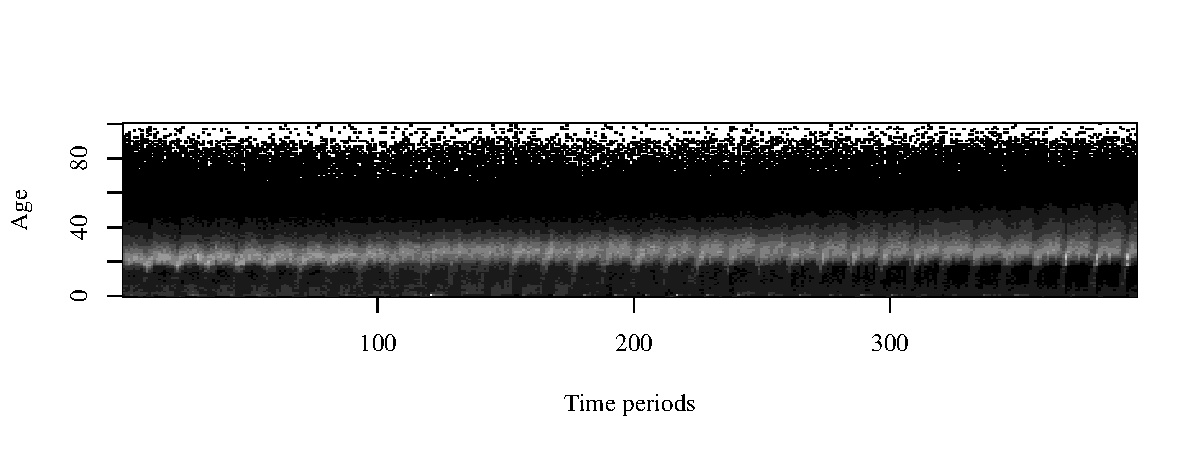
\includegraphics[width=\maxwidth]{figure/imageplot-1} \caption[Image plot showing migration frequencies, where dark gray indicates low frequency and light gray high frequency, by age from 01.01.1981 to 01.12.2013 (T=396)]{Image plot showing migration frequencies, where dark gray indicates low frequency and light gray high frequency, by age from 01.01.1981 to 01.12.2013 (T=396).}\label{fig:imageplot}
\end{figure}


\end{knitrout}



%%%%%%%%%%%%%%%%%%%%%%%%%%%%%%%%%%%%%%%%%%%%%%%%%%%%%%%%%%%%%%%%%%%%%%%%%%%%%%%%%%%%
%%%%%%%%%%%%%%%%%%%%%%%%%%%%%%%%%%%%%%%%%%%%%%%%%%%%%%%%%%%%%%%%%%%%%%%%%%%%%%%%%%%%
\subsection{Model Validation} \label{results}
%%%%%%%%%%%%%%%%%%%%%%%%%%%%%%%%%%%%%%%%%%%%%%%%%%%%%%%%%%%%%%%%%%%%%%%%%%%%%%%%%%%%
%%%%%%%%%%%%%%%%%%%%%%%%%%%%%%%%%%%%%%%%%%%%%%%%%%%%%%%%%%%%%%%%%%%%%%%%%%%%%%%%%%%%

The previous sections point out how the construction of a predictive model is performed at two stages: the analysis of the observed data and the incorporation of new available information. Hereafter we focus on both stages, first by undertaking a descriptive analysis of the immigration time series and then by elaborating suitable priors. 
The starting point is to decompose the logarithm of the number of monthly arrivals into a time and a seasonal trend, as in equation (\ref{decompose}), see Figure \ref{fig:decomposition}.

\begin{knitrout}
\definecolor{shadecolor}{rgb}{0.969, 0.969, 0.969}\color{fgcolor}\begin{figure}[!ht]
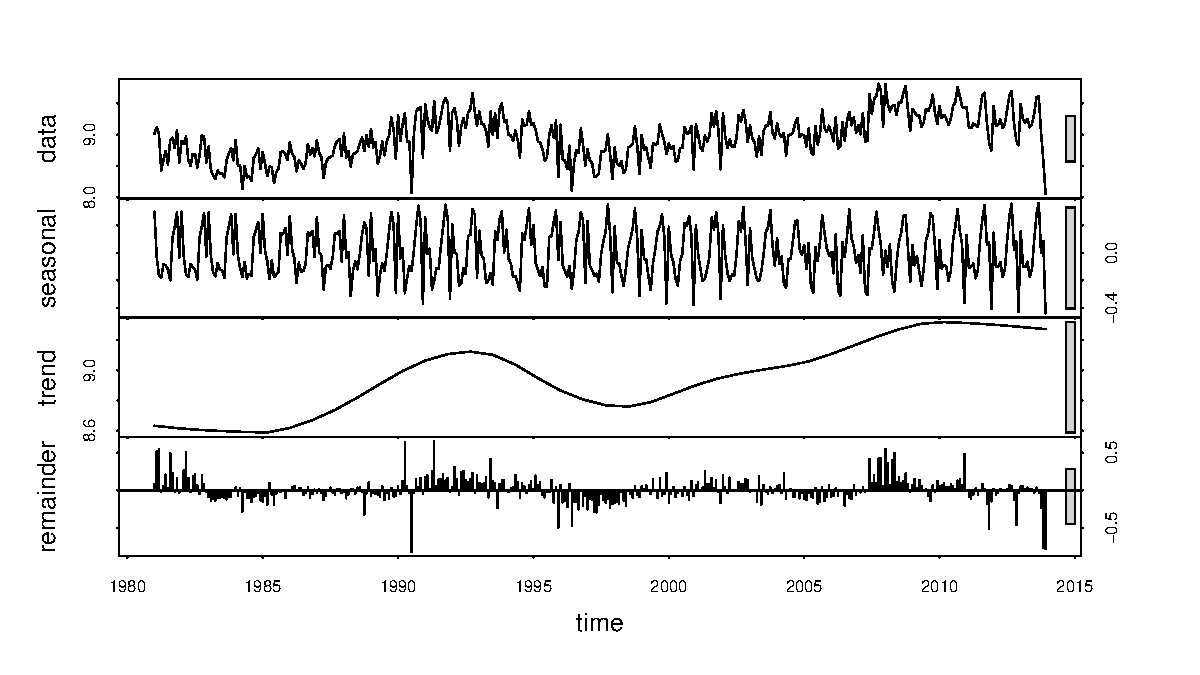
\includegraphics[width=\maxwidth]{figure/decomposition-1} \caption[Swiss Immigrant Flows Decomposition obtained using a locally weighted scatter-plot smoother (LOESS curve)]{Swiss Immigrant Flows Decomposition obtained using a locally weighted scatter-plot smoother (LOESS curve).  From the top to the bottom, the plots show: observed data, global trend, seasonal trend and random noise. }\label{fig:decomposition}
\end{figure}


\end{knitrout}

Given that the best trade trade-off between parsimony and accuracy is achieved with a 2nd order Fourier seasonality the reference model with interaction becomes,
\begin{align}\label{fourier_2nd_lm}
y_{t}= \beta_0 + \beta_1 \text{trend}_t + \sum_{i=1}^2 \beta_{2i} (\cos_{it} + \sin_{it}) + \sum_{i=1}^2 \beta_{3i} \text{trend}_t* (\cos_{it} + \sin_{it}) + \epsilon_{t}.
\end{align}
For the coefficients of equation (\ref{fourier_2nd_lm}) we use as prior a multivariate normal distribution,  
\begin{align}\label{matrix prior2}
\begin{bmatrix}
\beta_{0} \\
\beta_{1}\\
\beta_{21}\\
\beta_{22}\\
\beta_{31} \\
\beta_{32} 
\end{bmatrix}
\sim N
\begin{bmatrix}
\begin{pmatrix}
9 \\
0 \\
0 \\
0 \\
0 \\
0 
\end{pmatrix}
,
\begin{pmatrix}
0.5 & 0 & 0 & 0 & 0 & 0  \\ 
0 & 0.5 & 0 & 0 & 0 & 0  \\
0 & 0 & 0.5 & 0 & 0 & 0  \\
0 & 0 & 0 & 0.5 & 0 & 0  \\
0 & 0 & 0 & 0 & 0.5 & 0 \\
0 & 0 & 0 & 0 &  0  & 0.5
\end{pmatrix}
\end{bmatrix},
\end{align}
where the mean of the intercept has been set to 9, which is the average value of the logarithm of the immigration for the observed periods, while the standard deviation is 0.5 since we are confident that the mean can be neither lower than 7.4 nor higher than 10.6. The mean of the other coefficients is centered on 0 with a standard deviation of 0.5. This choice imposes the means of the $\beta$s of global trend, sine, cosine and trend-(sin+cos) interaction to be between -2 and 2. Note that the absence of covariance between the different coefficients allows to vectorize the prior and speed up the convergence rate of the algorithm. The same prior is used for the only coefficient of the equivalent additive model,
\begin{align}\label{fourier_2nd_gam}
y_{t}=\beta_{0}+ f_{1}(\text{trend}_{t})+\sum_{i=1}^{2}f_{2i}(\cos_{it}+\sin_{it})+\sum_{i=1}^{2}f_{3i}(\text{trend}_{t}, \cos_{it}+\sin_{it})+\epsilon_{t},
\end{align}
such that $\beta_0 \sim N(9, 0.5)$. The coefficients which identify the splines are assumed to be normally distributed with variances equal to 1, while the priors of the standard deviation of the error and of $\lambda$ are set to half Cauchy, see \citeA{StanPrior}, 
\begin{align}\label{variance}
\sigma_{\epsilon} \sim HC(0,2) \quad \quad \sigma_{\lambda} \sim HC(0,2).
\end{align}

Therefore, the coefficients' priors should be considered as empirical informative, while the variances' ones weakly informative, see Figure \ref{fig:weak priors}.

\begin{knitrout}
\definecolor{shadecolor}{rgb}{0.969, 0.969, 0.969}\color{fgcolor}\begin{figure}[!ht]
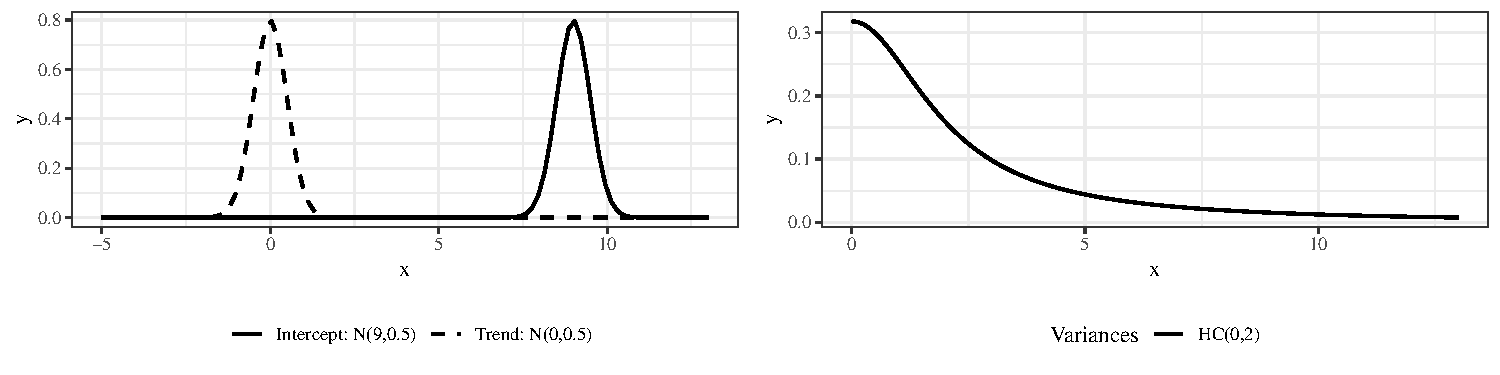
\includegraphics[width=\maxwidth]{figure/weak_priors-1} \caption[Representation of the priors for the coefficients and the variances]{Representation of the priors for the coefficients and the variances.}\label{fig:weak priors}
\end{figure}


\end{knitrout}

%We decided to choose a conservative prior for the intercept, relying on the average global trend, and to let the deviation from such mean, as well as the amplitude of the seasonal cycles greater margins of variability. This decision was mainly due to stabilize a part of the estimation. In fact the logarithm of the observed immigration series rages from a minimum of 8.054 to a maximum of 9.816 with a mean of 8.963. 
Given the aim of our analysis, we need to check which of the specifications presented in section \ref{methodology} produces the best forecasts. The first step in this direction requires to split the data into two subsets. The \textit{training data} (from January 1981 till December 2003) are used to fit the model, and the \textit{test data} (from January 2004 till December 2013), are used to predict the immigration flows. Once this first comparison has been done, it is possible to check the forecast's accuracy. Table \ref{RMSFE} reports three standard measures to compare the \textit{ex post} average forecast with the observed values.



 
\begin{table} \centering 
\caption{2nd order Fourier models on Swiss Immigration Aggregated Data for Short and Long Run Predictions.} 
\label{RMSFE} 
\resizebox{\columnwidth}{0.1\textheight}{
  \begin{tabular}{@{\extracolsep{5pt}}lcccccccc} 
  \\[-1.8ex]\hline 
  \hline \\[-1.8ex] 
&  \multicolumn{4}{c}{Short Run Predictions}&\multicolumn{4}{c}{Long Run Predictions} \\
\cline{2-5} \cline{6-9}  \\
&  \multicolumn{1}{c}{RMSFE}&\multicolumn{1}{c}{MAPE} &\multicolumn{1}{c}{95\%}&\multicolumn{1}{c}{90\%}
&  \multicolumn{1}{c}{RMSFE}&\multicolumn{1}{c}{MAPE} &\multicolumn{1}{c}{95\%}&\multicolumn{1}{c}{90\%} \\
  \hline \\[-1.8ex] 
LMNI           & 0.324 & 0.029 &  94  & 88   & 0.293 & 0.025 &  98 &  94    \\  % 2nd
AMNI           & 0.281 & 0.023 &  98  & 94   & 0.281 & 0.024 &  98 &  94    \\ % 2nd
LMI            & 0.324 & 0.029 &  94  & 88   & 0.287 & 0.025 &  99 &  96    \\ % 2nd
AMI            & 0.260 & 0.022 &  89  & 94   & 0.270 & 0.023 &  99 & 95.5   \\ % 2nd
NPM            & 0.586 & 0.060 &  50  & 39   & 1.572 & 0.183 &  21 &  17    \\ % 2nd

  \hline 
  \hline \\[-1.8ex] 
  \end{tabular}
} 
\end{table}


According to the RMSFE and the MAPE the AMI emerges as the most accurate model followed by the AMNI, the two linear models, LMNI and LMI, and far behind the NPM. Also in terms of Credible Intervals (CI) the AMI and the AMNI achieve the best coverage with a 98\% for the 95\% CI and a 94\% for the 90\% CI. The poor performance of the NPM seems driven by the usual overfitting of non-additive models. Such specification returns a decreasing trend, while the observed one is increasing. The results' comparison between AMNI and NPM suggests that, in the Swiss data, the necessity of modelling the trend is stronger than the one of the interaction. Nevertheless, a certain degree of non-linear trend-seasonal interplay is still present making the AMI the best predictive model. Figure \ref{fig:prediction} visually portrays the gains quantitatively evaluated in Table \ref{RMSFE}. More detailed results are given in the Additional Material \\

\begin{figure}[H]
\centering
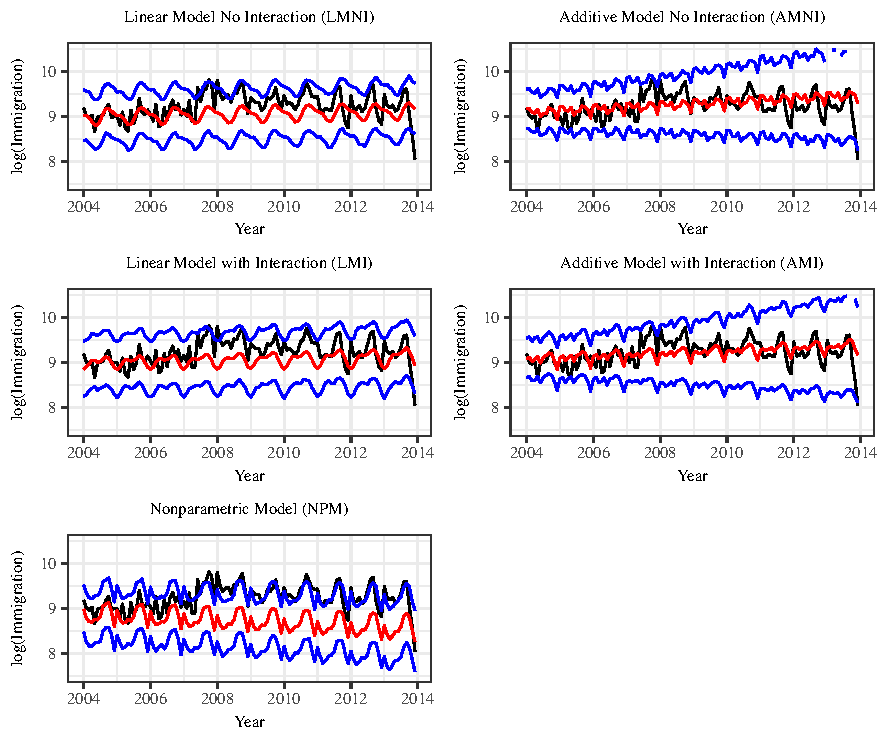
\includegraphics[scale=1]{Short_run_rsults.pdf}
\caption{Aggregated forecasts 2004-2013 with $95\%$ prediction credible interval from the posterior predictive distribution.}
\label{fig:prediction}
\end{figure}


Nonetheless, the short time horizon chosen to implement the forecasts might influence the performance results' in favor of the semiparametric models. In fact, the smooth trend term is computed using a piece-wise regression where the \textit{optimal} number of knots is obtained from the training, not the testing data. Therefore, in presence of a highly non-linear trend, the number of knots might be quite high. While this could be of no particular problem in the short run, when the probability of maintaining a trend close to the one of the last periods is realistic, in the long run this might be more problematic. Hence, a safer choice is either to use a low number of knots or to substitute $f_1(\cdot)$ with a parametric component in order to stabilize the semiparametric tendency to overfit out-of-sample forecasts, such that the AMNI becomes,
\begin{align}\label{fourier_gam_no_int_long}
y_{t}=\beta_{0}+\beta_{1}\text{trend}_{t}+\sum_{i=1}^{2}f_{2i}(\cos_{it}+\sin_{it})+\epsilon_{t},
\end{align}

while the AMI is,

\begin{align}\label{fourier_gam_int_long}
y_{t}=\beta_{0}+\beta_{1}\text{trend}_{t}+\sum_{i=1}^{2}f_{2i}(\cos_{it}+\sin_{it})+\sum_{i=1}^{2}f_{3i}(\text{trend}_{t}, \cos_{it}+\sin_{it})+\epsilon_{t},
\end{align}

and the NPM
\begin{align}\label{fourier_non_par_long}
y_{t} = \beta_{0} + \beta_{1}\text{trend}_{t} + f\bigg(\text{trend}_t, \sum_{i=1}^{2} (\cos_{it} + \sin_{it}) \bigg) + \epsilon_{t}.
\end{align}

The results show that the long term predictions highly benefit from a linear trend reducing the RMSFE by 600\% and the MAPE by 900\%. Note that the addition of the parametric term $ \beta_{1} $ is strictly related to the proposed estimation technique, i.e. the thin plate regression splines. If, for example, $ f_{1}(.) $ would have been estimated using a local polynomial approximation the required stabilization would have been embodied in the estimation methodology. 
%Since the introduction of $ \beta_{1} $ stabilizes the forecast, it is possible to use an even less informative prior for the variance of nonparametric part of the model. Among the different possibilities we use an half normal HN(0,0.3) which is smoother than the previously proposed half Cauchy HC(0,2) as shown in the dotted curve in the left hand plot of Figure \ref{fig:weak priors 1}. 
The results for the forecast period 1998-2013 mainly reflect the ones of the shorter term, with a slight improvement of the LMI over the LMNI. In general, both time horizons show a premium for the AMI specification. It is also interesting to notice how the NPM still overfits the data regardless the additional linear trend term.

\begin{figure}[H]
\centering
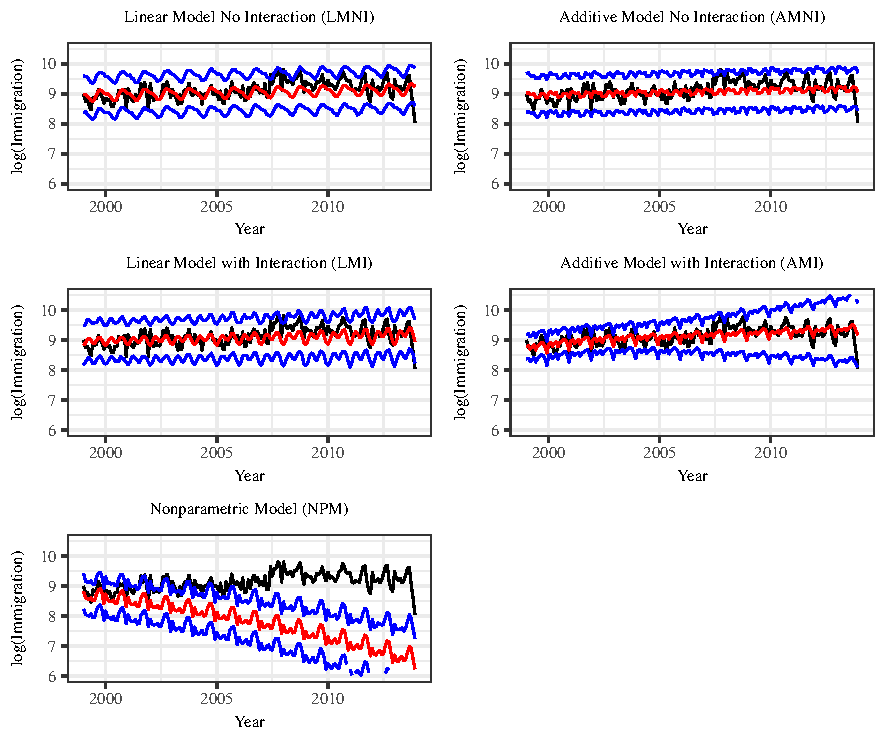
\includegraphics[scale=1]{Long_run_rsults.pdf}
\caption{Forecasts 1998-2013 with $95\%$ prediction credible interval from the posterior predictive distribution.}
\label{fig:prediction new horizons}
\end{figure}




A closer look to the reminders plotted at the bottom of Figure \ref{fig:decomposition} may suggest the presence of autocorrelation among the residuals. Potentially, such autocorrelation might persist also in the residuals of the LMNI, AMNI, LMI, AMI and NPM models. Hence, we try to re-estimate all the models, both for the short and the long run, by allowing their residuals to be autocorrelated of order 1 (AR(1)):

\begin{align}\label{AR(1)}
\epsilon_{t} = \alpha \epsilon_{t-1} + \xi_{t}, \quad -1 < \alpha < 1, \quad \xi_{t} \sim N(0,\sigma_{\xi}^2).
\end{align}

Table \ref{RMSFE AR1} confirms an improvement in prediction accuracy with a reduction of the RMSFE of 11\%, of the MAPE of 33\% and an extra coverage of the 95\% and 90\% credible intervals of respectively of 1.3\% and 15\%. The amelioration can also be traced in Figures \ref{fig:prediction AR(1) short} and \ref{fig:prediction AR(1) long}. In general models' performances are in line with the one of Table \ref{RMSFE}. However, the comparative advantage of the AMI with respect to the LMI, while being improved in the long run, is reduced for the short run. 
A possible explanation can be found in the origin of the autocorrelation among errors. For example, if there are logarithmic or exponential terms in the data generatin process, the LMs would most probably generate autocorrelated errors. Therefore, equation \ref{fourier_2nd_lm} benefits from the introduction of (\ref{AR(1)}). To the contrary, the AMs, by construction, tend to solve autocorrelation generated by functional form misspecifications, gaining less from the inclusion of an AR(1) component. Figure \ref{fig:residuals} shows how the LMI reports stronger evidence of residuals dependence than the AMI\footnote{
A Box-Pierce test statistic for examining the null hypothesis of independence of the residuals is rejected with a p-value < 2.2e-16 for the LMI and a p-value = 0.0022 for the AMI.
}. 

%Mean RMSFE 0.2898
%Mean RMSFE AR(1) 0.257
%Average improvement RMSFE: -0.1131815
%Mean MAPE 0.0326
%Mean MAPE AR(1) 0.0222
%Average improvement MAPE: -0.3251534
%Mean 95% coverage 85
%Mean 95% coverage AR(1) 96.3
%Average improvement 95% coverage: 1.3%
%Mean 90% coverage 80.6
%Mean 90% coverage AR(1) 92.8
%Average improvement 90% coverage: 15%


\begin{table} \centering 
\caption{2nd order Fourier models on Swiss Immigration Aggregated Data for Short and Long Run Predictions with AR(1) errors.} 
\label{RMSFE AR1} 
\resizebox{\columnwidth}{0.1\textheight}{
  \begin{tabular}{@{\extracolsep{5pt}}lcccccccc} 
  \\[-1.8ex]\hline 
  \hline \\[-1.8ex] 
&  \multicolumn{4}{c}{Short Run Predictions}&\multicolumn{4}{c}{Long Run Predictions} \\
\cline{2-5} \cline{6-9}  \\
&  \multicolumn{1}{c}{RMSFE}&\multicolumn{1}{c}{MAPE} &\multicolumn{1}{c}{95\%}&\multicolumn{1}{c}{90\%}
&  \multicolumn{1}{c}{RMSFE}&\multicolumn{1}{c}{MAPE} &\multicolumn{1}{c}{95\%}&\multicolumn{1}{c}{90\%} \\
  \hline \\[-1.8ex] 
LMNI           & 0.255 & 0.022 &  96    & 94   & 0.251 & 0.022 & 95 & 94    \\  % 2nd
AMNI           & 0.264 & 0.021 &  97.5  & 94   & 0.247 & 0.020 & 97 & 93    \\ % 2nd
LMI            & 0.248 & 0.021 &  96    & 93   & 0.252 & 0.021 & 97 & 94    \\ % 2nd
AMI            & 0.247 & 0.021 &  98    & 95   & 0.232 & 0.020 & 100 & 99  \\ % 2nd
NPM            & 0.271 & 0.026 &  94    & 88   & 0.550 & 0.053 & 70 & 53    \\ % 2nd

  \hline 
  \hline \\[-1.8ex] 
  \end{tabular}
} 
\end{table}

\begin{figure}[H]
\centering
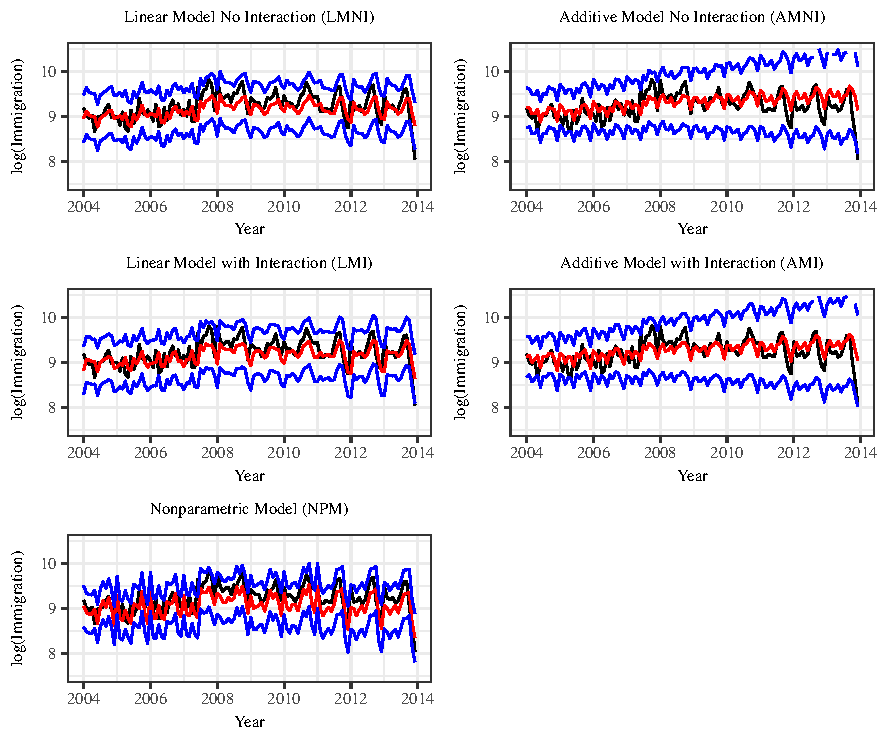
\includegraphics[scale=1]{Short_run_results_AR1.pdf}
\caption{Aggregated forecasts 2004-2013 with $95\%$ prediction credible interval from the posterior predictive distribution for models with autocorrelated residuals of order one (AR(1)).}
\label{fig:prediction AR(1) short}
\end{figure}

\begin{figure}[H]
\centering
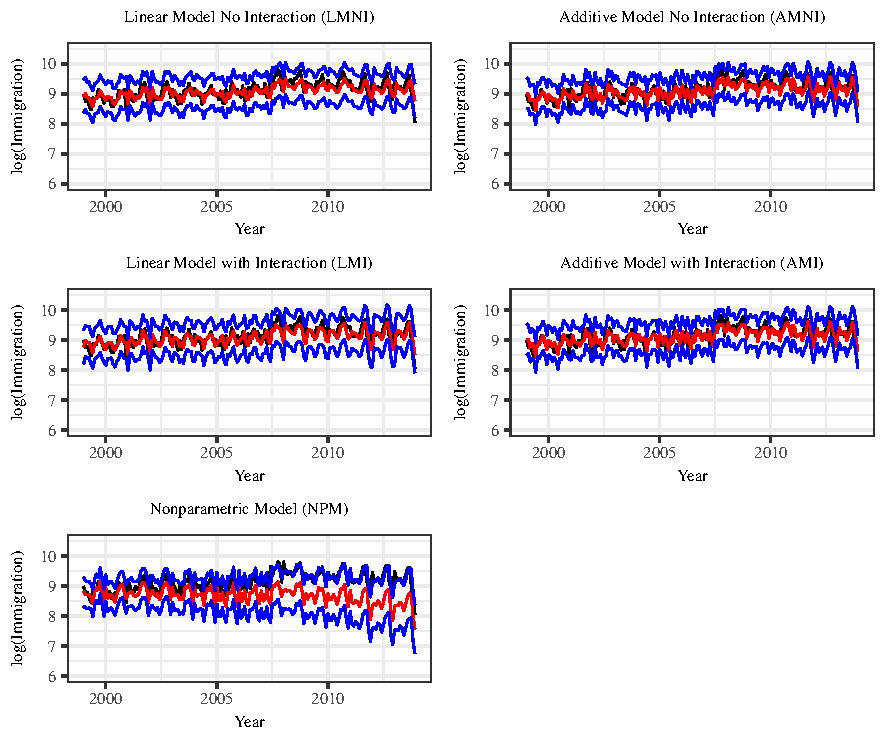
\includegraphics[scale=1]{Long_run_results_AR1.pdf}
\caption{Forecasts 1998-2013 with $95\%$ prediction credible interval from the posterior predictive distribution for models with autocorrelated residuals of order one (AR(1)).}
\label{fig:prediction AR(1) long}
\end{figure}

\begin{figure}[H]
\begin{minipage}{.5\textwidth}
\centering 
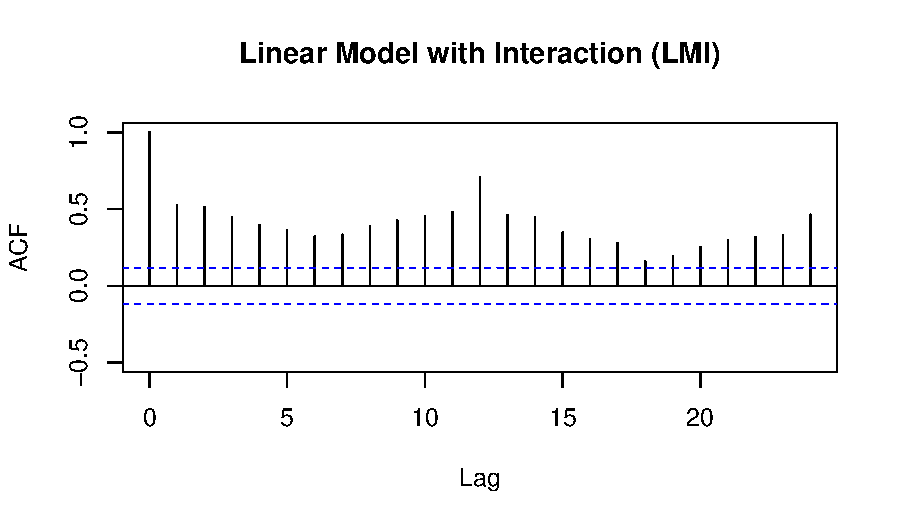
\includegraphics[scale=.5]{Residuals_LM_ST.pdf}
\end{minipage}
\begin{minipage}{.5\textwidth}
\centering 
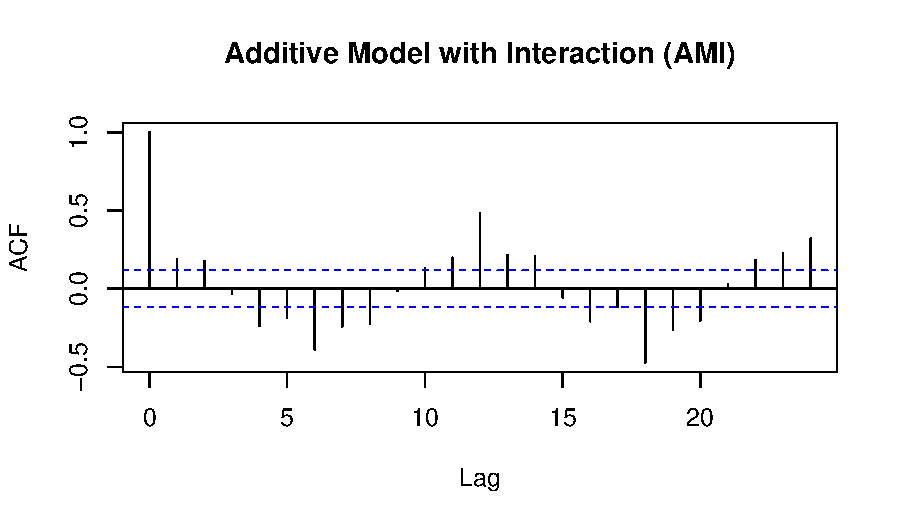
\includegraphics[scale=.5]{Residuals_AM_ST.pdf}
\end{minipage}
\caption{Estimates of the autocovariance or autocorrelation function for the linear model with interaction (left plot) and for the additive model with interaction (right plot).}
\label{fig:residuals}
\end{figure}

While the previous sections have shown how the semiparametric models tend to outperform the other alternatives both with simulated and historical data, we now illustrate how robust these results are with respect to the setting of different priors. \\
The first alternative is an uninformative prior defined over $ \mathbb{R} $ for $ \beta $ combined again with two standardized half t-student with three degrees of freedom for $\sigma_{\epsilon}$ and $\sigma_{\lambda}$ \cite{buerkner2016package}. A second possibility is to use the horseshoe hierarchical shrinkage prior with parameter 1 for $ \beta $ combined again with two standardized half t-student for the variances of $ \epsilon $ and $ \lambda $. The outcomes confirm that the AMI is robust to these alternative specifications, see Figure \ref{fig:comparison}.





\begin{figure}[H]
\centering
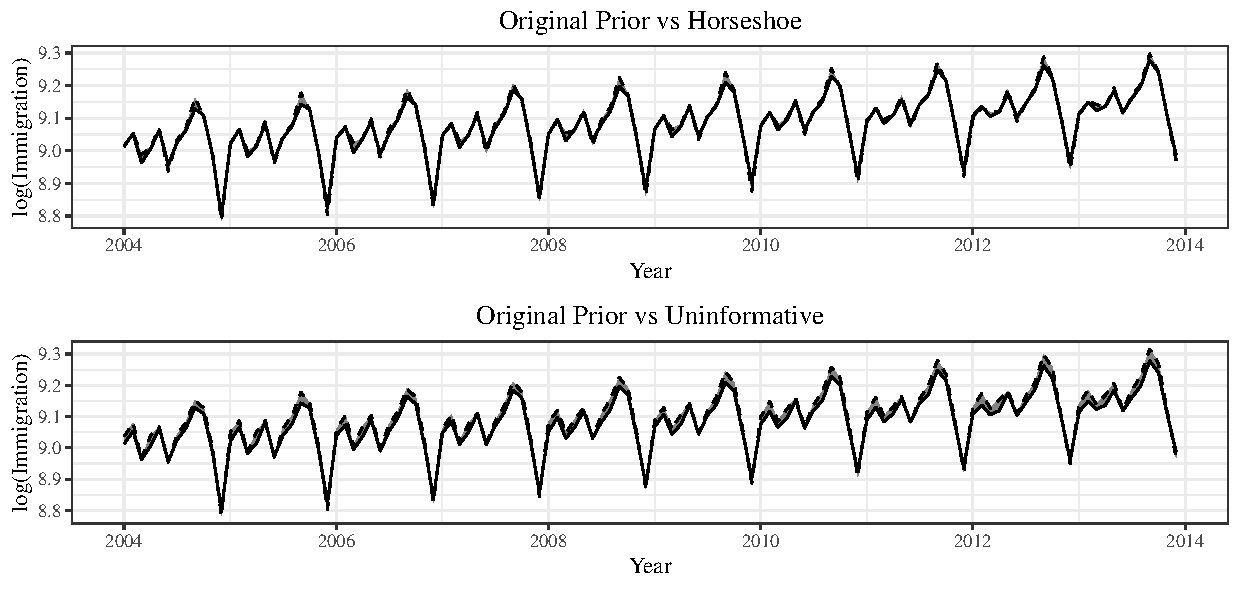
\includegraphics[scale=0.7]{forecasts_comparison.pdf}
\caption{Priors' robustness comparison for the predictions over the period 2004-2014. The black line denotes the forecasts obtained with the original prior distributions used in the analysis. The red lines are the forecasts obtained with comparative priors, the horseshoe in the top and the uninformative in the bottom plot. The difference is the blue area.}
\label{fig:comparison}
\end{figure}

So far we have shown how the Bayesian Additive Model with Interaction outperforms the alternatives in predicting the behaviour of the test data starting from the fit of the training data. However, our argument in favour of Bayesian statistics was rooted in its capacity to introduce informative believes through the choice of the prior distributions. Therefore, we propose, in the next Subsection, an illustrative example which directly shows the advantages of adopting different priors in the predictions.

\subsection{Forecast Exercise}\label{forecast}

In this subsection we fit the AMI on the Swiss data for all the available years (1981-2013) and we try to forecast immigration flows until 2023. %The forecasts make an active use of the priors, setting up alternative scenarios reflecting different expectations. 
Since the priors are used, at the same time, to estimate the model and, indirectly, to implement the forecasts, their distributions link historical knowledge with future expectations. Therefore, if migration is foreseen to look like the past, flat priors with relatively high variances should be chosen. To the contrary, if migration is anticipated to change, informative priors, with smaller variances around the expected means should be selected. The latter case, however, may give room to divergent transitions within the sampling. \\ 
For this study we set up three scenarios. The first pictures the sentiment of a future migration in line with its historical average.
Therefore, it relies on weakly informative priors. For example, the intercept's prior takes the same values as in the model validation exercise with a mean of 9 and a standard deviation of 0.5. In the same way, the trend's prior is centered around the posterior obtained from section \ref{results}, but with a wider variance to convey a minimal impact on its posterior distribution. 
The second scenario is a middle story line, which reflects the possibility of a small shock. In this case, the trend's prior is centered around 1.5, rather than 0, with a variance of 0.2, which suggests an increased return of the trend. 
The third is a scene, which mirrors the expectation of a more evident structural break on the trend's historical impact on $y_{t}$. This last case is achieved by increasing the expected mean up to 2, while shrinking its variance to 0.1.   \\*
In order to make sure that the difference between the three scenarios is only about the researcher's expectations about structural changes we do not modify the priors for the standard deviation of the error term ($\sigma_{\xi}$) and of the smoothing parameter ($\sigma_{\lambda}$) assuming that in every case they are distributed as Half-Cauchy with a scale parameter of 2, like in section \ref{results}.
Instead, we play mostly with the priors of the error's autocorrelation term ($\alpha$) assuming increasing path dependency coherently following the discussion on the trend's priors. 
All the distributions are described in Table \ref{prior distribution 1} and portrayed in Figure \ref{fig:posteriors vs priors}.








\begin{figure}[H]
\centering
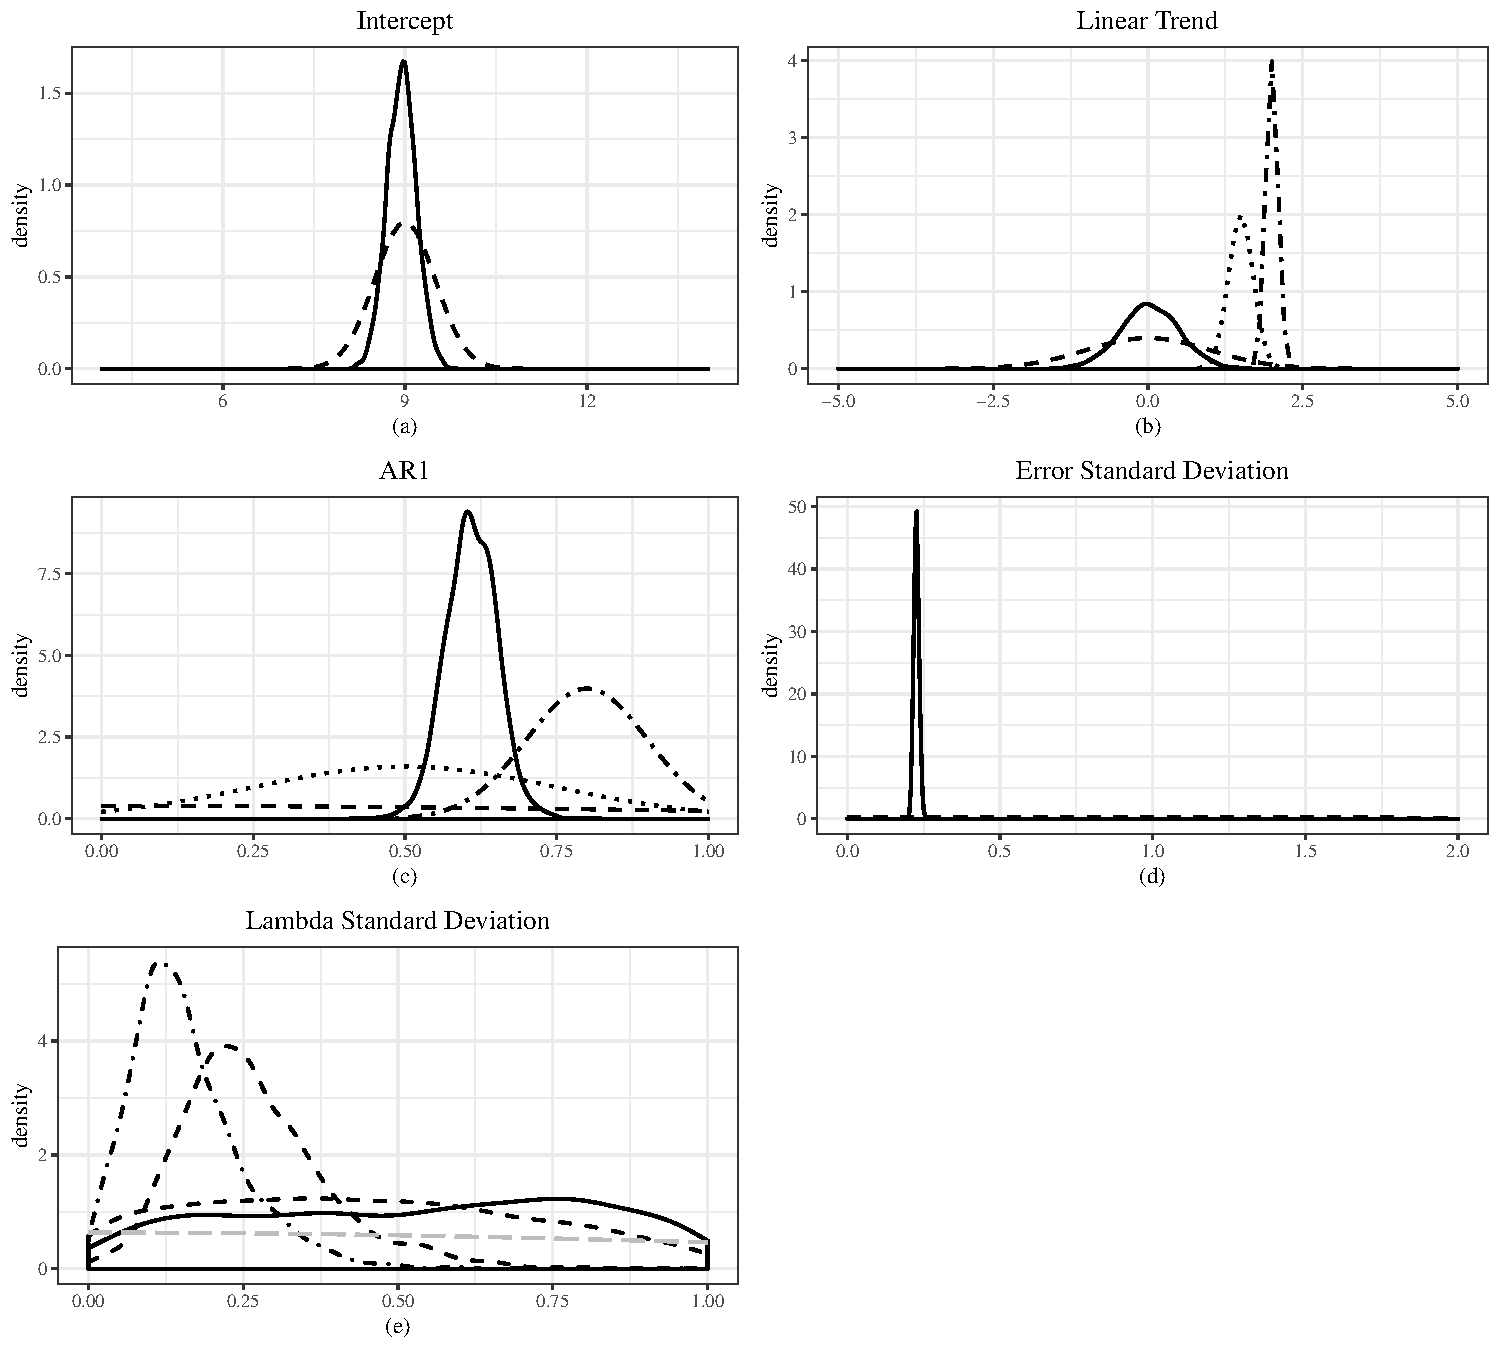
\includegraphics[scale=0.6]{posterior.pdf}
\caption{The plots compare the posterior distributions obtained from the AMI with autoregressive errors of order one for the period 1981-2013 (solid line) with the priors chosen to set the different forecast scenarios (dashed and dotted lines). From top to bottom and left to right the graphs show the distributions for the intercept, the linear trend's coefficient, the error autoregressive coefficient (AR1), the error's standard deviation and the standard deviation of the smoothing parameter.}
\label{fig:posteriors vs priors}
\end{figure}

\begin{table}[ht] \centering 
\caption{Prior Distributions for the Scenario Analysis} 
\label{prior distribution 1} 
\resizebox{.7\columnwidth}{0.08\textheight}{
  \begin{tabular}{@{\extracolsep{5pt}}lcccc} 
  \\[-1.8ex]\hline 
  \hline \\[-1.8ex] 
 & Historical Scenario & Middle Scenario & High Scenario \\  
  \cline{2-4} 
 \\[-1.8ex] 
$\beta_0$                   & N(9;0.5)    & N(9;0.5)      & N(9;0.5)  \\
$\beta_1$                   & N(0;1)      & N(1.5;0.2)    & N(2;0.1)  \\
$\alpha$                    & N(0;1)      & N(0.5;0.25)   & N(0.8;0.1) \\
$\sigma_{\xi}$              & HC(0;2)     & HC(0;2)       & HC(0;2)  \\
$\sigma_{\lambda}$          & HC(0;2)     & HC(0;2)       & HC(0;2)  \\
  \hline 
  \hline \\[-1.8ex] 
  \end{tabular}
} 
\end{table}





For each scenario we model the global trend in three different ways. The choice stems from the reasoning already presented in the previous sections, where we outlined the potential problems raising from a smooth trend with a considerable number of knots for long term forecasts. Thus, the three models include as alternatives a linear trend ($\beta_{1}\text{trend}_{t}$) and two smooth trends with respectively four, $f_{1}(\text{trend}_{t}, \text{k}=4)$, and six knots, $f_{1}(\text{trend}_{t}, \text{k}=6)$. The difference in the results is more visible for the trend fitted on six knots, especially in the case of historical and middle scenarios, where the global trend is down-warding. In general when the trend is nonparametrically computed with k=6, the average future immigration is approximately 40\% lower than in the linear case for the historical and the middle scenario.   \\* 
In the historical scenario, the median number of immigrants rises from its historic value of 99,070 people per year to 147,646 for the linear trend, to 206,151 for the smooth trend with k=4 and shrinks to 82,701 for the smooth trend with k=6, showing respectively an increase of 49\% and 68\% and a decrease of 17\%. In the middle scenario the median number of immigrants becomes 148,313 for the linear trend, 185,752 for the smoothing trend with k=4 and 109,584 for k=6 corresponding respectively to a 50\%, 87\% and 11\% increase. Finally, the high scenario finds a growth rate of 53\% for the linear trend, of 168\% for the smoothing trend with k=4 and of 136\% for k=6. Figure \ref{fig:forecast scenarios} visualizes the results. Note that all the growth rates would be down-sized if we would look at the median immigration of the last 10 and 5 years rather than the one from 1981 till 2013. \\*

\begin{figure}[H]
\centering
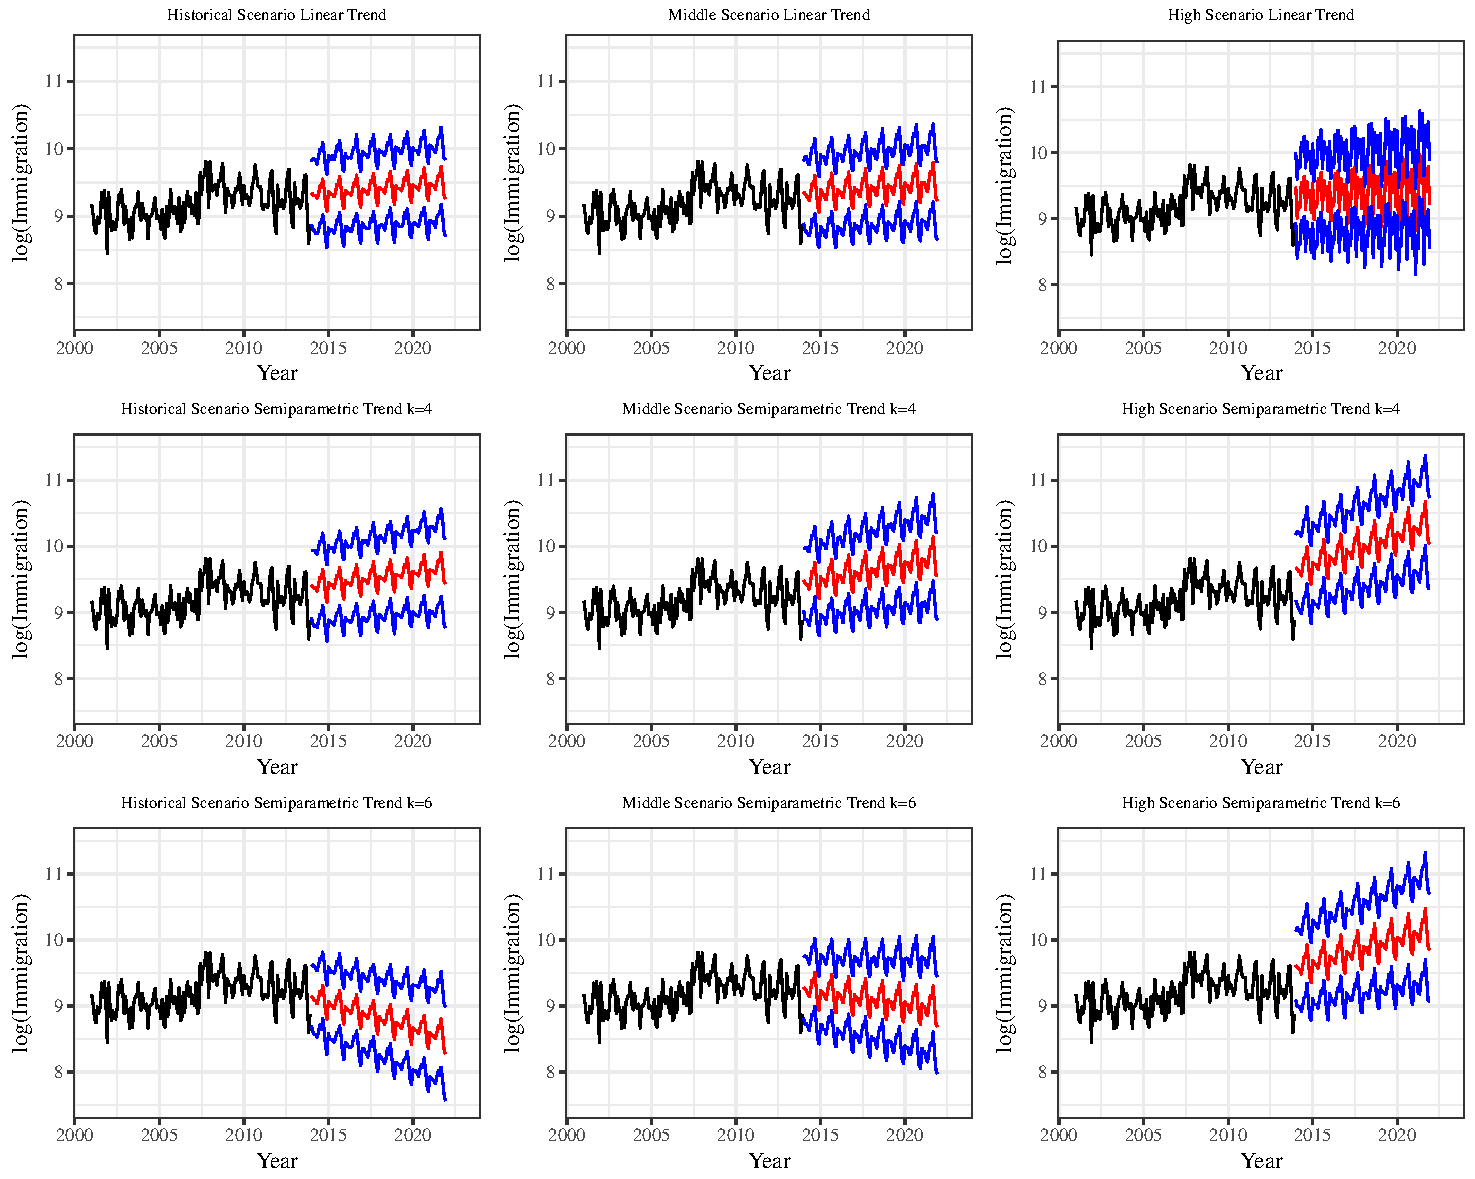
\includegraphics[scale=0.6]{Forecast_results_new.pdf}
\caption{Forecasts 2013-2021 with $95\%$ prediction credible interval from the posterior predictive distribution for three different priors.}
\label{fig:forecast scenarios}
\end{figure}

As a general remark from our forecast exercise, practitioners should be careful in treating the global trend either parametrically or nonparametrically, as well as, in the degree of volatility conveyed by the priors. 
In general a large number of knots requires more coefficients (one for each knots interval) and, consequently, a loss in degrees of freedom. Said differently, including an excessive number of knots reduces the degrees of freedom available to estimate the parameters' variability, potentially having a negative impact on the forecast's quality. 
Furthermore, since the paper stresses the benefits of modelling semiparametrically the trend-seasonal interaction, estimating the trend in  parsimonious ways allows to devote a larger number of degrees of freedom to fit the interaction without worsening the prediction accuracy.


\section{Longitudinal Analysis of Age Categorized Data} \label{disaggregated results}
\subsection{Model Validation} \label{model_disaggregation}

To illustrate the adaptability of our model to a disaggregated problem we employ longitudinal data categorizing the monthly number of arrivals by age. Further distinctions by gender or nationality can, at any rate, be implemented, but they are not considered here. \\
Splitting our data into different ages allows us to check the persistence of non-linearity and trend-cycle interactions. We add  $Age$ as an explanatory variable to the models estimated for the time series. The latter is introduced as a parametric term, $\beta_4 Age_{age,t}$, in LMNI and LMI, as a smooth function $ f_{4}(Age_{age,t})$ in AMNI and AMI \shortcite{dodd2018smoothing}, while for the the nonparametric model (NPM), we add it to the main smoothing function $f$. To estimate the Bayesian models we adopt the same priors as in the aggregate exercise, with in addition $\beta_4 \sim N(0,0.5)$. 
%The models are transformed in the following way to accommodate the longitudinal format,
%\begin{align*}
%\text{LMNI}: \\
%y_{age,t}&= \beta_0 + \beta_1 \text{trend}_{age,t} + \sum_{i=1}^2 \beta_{2i} (\cos_{it} + \sin_{it}) + \beta_4 Age_{age,t}+ \epsilon_{t}, \\
%\text{LMI}: \\
%y_{age,t}&= \beta_0 + \beta_1 \text{trend}_{age,t} + \sum_{i=1}^2 \beta_{2i} (\cos_{it} + \sin_{it}) + \sum_{i=1}^2 \beta_{3i} \text{trend}_{age,t}*(\cos_{it} + \sin_{it}) + \beta_4 Age_{age,t} + \epsilon_{t}, \\
%\text{AMNI}: \\
%y_{age,t}&= \beta_{0} + f_{1}(\text{trend}_{age,t}) + \sum_{i=1}^{2} f_{21} (\cos_{it} + \sin_{it}) + f_{3}(Age_{age,t}) + \epsilon_{t}, \\
%\text{AMI}: \\
%y_{age,t}&=\beta_{0}+ f_{1}(\text{trend}_{age,t}) + \sum_{i=1}^{2}f_{2i}(\cos_{it} + \sin_{it}) + \sum_{i=1}^{2}f_{3i}(\text{trend}_{t}, \cos_{it} + \sin_{it}) + f_{3}(Age_{age,t}) + \epsilon_{t}, \\
%\text{NPM}: \\
%y_{age,t}&= \beta_{0} + f\bigg(\text{trend}_{age,t}, \sum_{i=1}^{2} (\cos_{it} + \sin_{it}), Age_{age,t} \bigg) + \epsilon_{t}, 
%\end{align*}

%where $ \epsilon_{age, t} \sim N(0, \sigma_{\epsilon}^2) $ and $Age_{age,t}$ is the migrants' age. 




The results in Table \ref{RMSFE_age}  show an increase in uncertainty produced by the disaggregation. On average the RMSFE increases by 130\% and the MAPE by 770\%.  The improvements given by the use of semiparametric and nonparametric models are reinforced, dropping the RMSFE from 1.16 (LMNI, LMI) to 0.66 (AMNI, AMI) and to 0.54 (NPM). However, the relative forecast accuracy measure, the mean absolute percentage error, portrays a different picture. The AMNI and the AMI achieve the most precise predictions with a MAPE of 0.24, followed by the LMNI and the LMI with a MAPE of 0.31 and lastly by the NPM with a MAPE of 0.33. The difference reflects the specific peculiarities of the absolute (RMSFE) vs the relative (MAPE) accuracy measures. In our case the NPM is doing better than the alternatives in minimizing the big error generated by the predictions of outlier observations, i.e. low RMSFE, but it produces a poorer performance, on average, when predicting smaller values, i.e. high MAPE. On the other hand, AMNI and AMI minimize the errors between, let say 0.11 and 0.12 rater than the ones between 0.81 and 0.82. In light of such considerations, the semiparametric models seem a more cautious choice over the nonparametric one. \\
In general, the disaggregation, while it does not generate any significant linearization, confirming the better performance of the semiparametric models, it minimizes the importance of the trend-seasonal interaction, which is reflected in the absence of a significant difference between the models with and without it. 

\begin{table}
\centering
\caption{2nd order Fourier models on Swiss Immigration Disaggregated Data: Root Mean Square Forecast Error (RMSFE) and Mean Average Percentage Error (MAPE) and prediction interval coverage}
\label{RMSFE_age} 
\resizebox{.5\columnwidth}{0.08\textheight}{
  \begin{tabular}{@{\extracolsep{5pt}}lcccc} 
  \\[-1.8ex]\hline 
  \hline \\[-1.8ex] 
&  \multicolumn{1}{c}{RMSFE}&\multicolumn{1}{c}{MAPE} &\multicolumn{1}{c}{95\%}&\multicolumn{1}{c}{90\%} \\
  \hline \\[-1.8ex] 
LMNI           & 1.165 & 0.314 &  95  & 81      \\  % 2nd
AMNI           & 0.662 & 0.245 &  89  & 79.5          \\ % 2nd
LMI            & 1.165 & 0.314 &  95  & 81     \\ %2nd
AMI            & 0.662 & 0.246 &  90  & 79       \\ % 2nd
NPM            & 0.547 & 0.330 &  91  & 83       \\ % 2nd

  \hline 
  \hline \\[-1.8ex] 
  \end{tabular}
} 
\end{table}


\subsection{Forecast Exercise}\label{disaggregated forecast}

The previous section validates the additive models as the preferable options to predict future immigration flows by age. This section presents a forecast exercise on the Swiss data for the period 2014-2021, which replicates the one in section \ref{forecast}, for the longitudinal case. Even though the difference between the AMNI and the AMI is not particularly relevant, we use the AMI, not only to keep a certain degree of consistency with section \ref{forecast}, but also because the AMI has a faster rate of convergence. Using the same priors as in the time series analysis, see Table \ref{prior distribution 1}, we check the performances of different trends: linear, smooth with three (k=4) and six (k=6) knots. Figure \ref{fig:trend comparison} reports the results under the low volatility scenario averaged over all the forecast periods. While the linear and the smooth trend with three knots have a very similar behaviour, the smoothest trend suffers from the same down-ward trend as in the aggregate case portrayed in Figure \ref{fig:prediction}. Due to the non significant difference between the blue (linear) and the red (k=4) line, we use the former to produce the disaggregated forecast scenario analysis. 

\begin{figure}
\centering
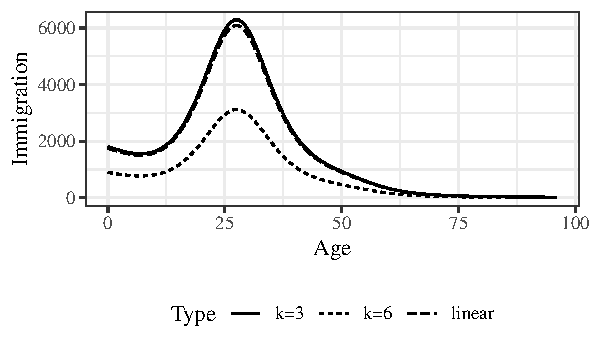
\includegraphics[scale=1]{Plot_trend_dis.pdf}
\caption{Effect of a different trend specification on the predictions of age-specific immigration forecast with on the y-axis the average yearly number of immigrants for the predicted period (2014-2021) and on the x-axis the age. The blue line denotes the results obtained with a linear trend, the red one with a smooth trend with 3 knots (k=4) and the green one with a smooth trend with 6 knots (k=6).}
\label{fig:trend comparison}
\end{figure}

The results are depicted in Figure \ref{fig:forecast age}. In all the three cases, the expected amount of immigration by age resembles a normal distribution centered around 33, with a third moment bigger than zero. All the scenarios roughly maintain the same immigrant population age structure as the historical data. Nevertheless, as volatility increases, the degree of smoothness decreases. The same is true as the forecast horizon augments. \\
A final remark that needs to be made when considering disaggregated forecasts is how to manage the "pooling-back" when the final interest is to know the future of Swiss migration as a whole. In fact, stacking the average forecasts by age implies also stacking the credibility intervals which might be difficult to handle and risk to degenerate in an uninformative explosion of uncertainty. In light of the results, while disaggregation is always a possibility, the age pooling seems a safer choice, which guarantees forecast accuracy, as well as stability.




\begin{figure}
\centering
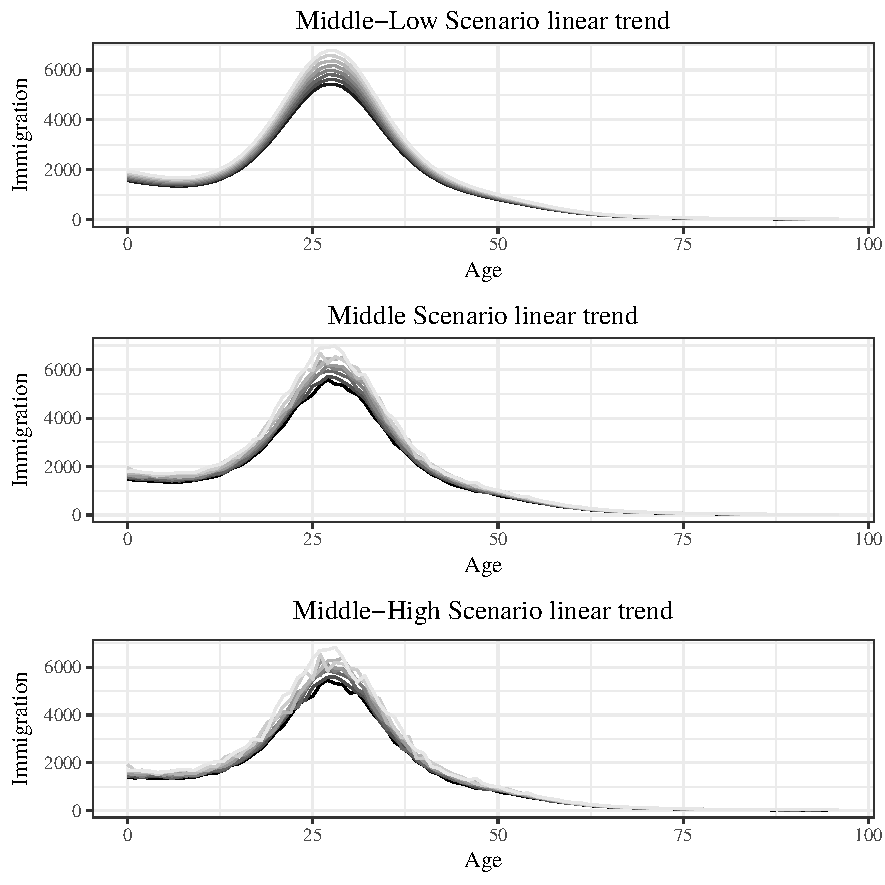
\includegraphics[scale=.8]{Plot_forecasts_age.pdf}
\caption{Disaggregated monthly forecasts averaged by year over the period 2014 (orange) - 2021 (pink) for three different scenarios from the posterior predictive distribution.}
\label{fig:forecast age}
\end{figure}


\section{Conclusion}\label{conclusion}
Migration gained the reputation of being an unpredictable component of population change \cite{pijpers2008problematising, bijak2010bayesian}. The current paper tries to show how merging Bayesian statistics with semiparametric methods can help to handle the uncertainty surrounding the number of future incomers. \\
The core of the research lies in the choice to consider migration as a seasonal, rather than an annual, phenomenon and to exploit the monthly frequency of the output to deal with eventual trend-seasonal interactions. Even if such focus limits the methodology's application to countries which dispose of high frequency data, it also potentially opens new perspectives for analyzing new migration trends, which show high seasonality, like the ones of the recent refugee crisis \shortcite{eu2017quantitative}.\\
%According to all the employed accuracy measures the AMI outperforms the competitors, even for age disaggregated data. \\
The message our results deliver is mainly twofold. On one side, the semiparametric models can represent an appealing alternative in presence of non-linear trend-cycle interactions. On the other, a Bayesian prospective can be proactively embraced through the choice of informative prior distributions to build forecast scenarios accounting for unprecedented events. The latter adds the possibility to condition the forecast on a set of macroeconomic projections \cite{bijak2010forecasting}. \\
Despite the model's choice belongs to the researcher discretionality, we have a few recommendations for future users in light of our investigation. Semiparametric models can be preferable in case of foreseen growing volatility since their flexibility can be fully exploited. However, they tend to exhibit increasing instability when dealing with long forecast horizons due to the usual overfitting of nonparametric models in out-of-sample performances. In such cases, a Bayesian perspective can help by setting boundaries on the prior distribution of the structural coefficients. 

%Migration gained the reputation of being an unpredictable component of population change \cite{pijpers2008problematising, bijak2010bayesian}. The current paper tries to show how merging Bayesian statistics with semiparametric methods can help to handle the uncertainty surrounding the number of future incomers. \\
%The core of the research lies in the choice to consider migration as a seasonal, rather than an annual, phenomenon and to exploit the monthly frequency of the output to deal with eventual trend-seasonal interactions. 

%Even if such focus limits the methodology's application to counries which dispose of seasonal data, it also potentially opens new prospectives for the analysis of new migration trends which show high seasonality like one of the recent refugee crisis.

%According to all the employed accuracy measures the AMI outperforms the competitors under weakly informative priors. \\
%The message our results delivers is mainly twofold. On one side, the semiparametric models can represent an appealing alternative in presence of non-constant trend-cycle interactions. On the other, a Bayesian prospective can be proactively embraced through the choice of informative prior distributions to build forecast scenarios accounting for unprecedented events. The latter adds the possibility to condition the forecast on a set of macroeconomic projections \cite{bijak2010forecasting}.\\ % The latter was somehow unexplored by the traditional migration forecasts which, instead, adopt a Bayesian approach mainly to deal with the lack of long data series or to make use of diffuse priors while using subjective believes to set threshold. \\
%It could be argued that the mix we proposed is appropriate only in the analysis of aggregated data while population forecasts are normally thought to deliver disaggregated results by gender and age. Therefore, we show how our procedure can outperform standard alternatives also for longitudinal datasets.\\ 
%Despite the model's choice belongs to the researcher discretionality, we have a few recommendations for future users in light of our investigation. Semiparametric models can be preferable in case of foreseen growing volatility since their flexibility can be fully exploited. However, they tend to exhibit increasing instability when dealing with long forecast horizons due to the usual limitations of nonparametric models in out-of-sample performances. In such cases, a Bayesian perspective can help by setting boundaries on the prior distribution of the structural coefficients.


\bibliography{Ref_proj}

\end{document}



















